% ******************************* PhD Thesis Template **************************
% Please have a look at the README.md file for info on how to use the template

\documentclass[a4paper,11pt,times,numbered,print,index]{Classes/PhDThesisPSnPDF}

% ******************************************************************************
% ******************************* Class Options ********************************
% *********************** See README for more details **************************
% ******************************************************************************

% `a4paper'(The University of Cambridge PhD thesis guidelines recommends a page
% size a4 - default option) or `a5paper': A5 Paper size is also allowed as per
% the Cambridge University Engineering Deparment guidelines for PhD thesis
%
% `11pt' or `12pt'(default): Font Size 10pt is NOT recommended by the University
% guidelines
%
% `oneside' or `twoside'(default): Printing double side (twoside) or single
% side.
%
% `print': Use `print' for print version with appropriate margins and page
% layout. Leaving the options field blank will activate Online version.
%
% `index': For index at the end of the thesis
%
% `draftclassic': For draft mode without loading any images (same as draft in book)
%
% `draft': Special draft mode with line numbers, images, and water mark with
% timestamp and custom text. Position of the text can also be modified.
%
% `abstract': To generate only the title page and abstract page with
% dissertation title and name, to submit to the Student Registry
%
% `chapter`: This option enables only the specified chapter and it's references
%  Useful for review and corrections.
%
% ************************* Custom Page Margins ********************************
%
% `custommargin`: Use `custommargin' in options to activate custom page margins,
% which can be defined in the preamble.tex. Custom margin will override
% print/online margin setup.
%
% *********************** Choosing the Fonts in Class Options ******************
%
% `times' : Times font with math support. (The Cambridge University guidelines
% recommend using times)
%
% `fourier': Utopia Font with Fourier Math font (Font has to be installed)
%            It's a free font.
%
% `customfont': Use `customfont' option in the document class and load the
% package in the preamble.tex
%
% default or leave empty: `Latin Modern' font will be loaded.
%
% ********************** Choosing the Bibliography style ***********************
%
% `authoryear': For author-year citation eg., Krishna (2013)
%
% `numbered': (Default Option) For numbered and sorted citation e.g., [1,5,2]
%
% `custombib': Define your own bibliography style in the `preamble.tex' file.
%              `\RequirePackage[square, sort, numbers, authoryear]{natbib}'.
%              This can be also used to load biblatex instead of natbib
%              (See Preamble)
%
% **************************** Choosing the Page Style *************************
%
% `default (leave empty)': For Page Numbers in Header (Left Even, Right Odd) and
% Chapter Name in Header (Right Even) and Section Name (Left Odd). Blank Footer.
%
% `PageStyleI': Chapter Name next & Page Number on Even Side (Left Even).
% Section Name & Page Number in Header on Odd Side (Right Odd). Footer is empty.
%
% `PageStyleII': Chapter Name on Even Side (Left Even) in Header. Section Number
% and Section Name in Header on Odd Side (Right Odd). Page numbering in footer

% Uncomment to change page style
%\pagestyle{PageStyleII}

% ********************************** Preamble **********************************
% Preamble: Contains packages and user-defined commands and settings
% ******************************************************************************
% ***************************** Custom Packages ********************************
\usepackage{physics}
\usepackage{graphicx}
\usepackage[pdftex,dvipsnames]{xcolor}  % Coloured text etc.
\usepackage[colorinlistoftodos,prependcaption,textsize=tiny]{todonotes}
\usepackage{xspace}
\usepackage{hyperref}
\hypersetup{colorlinks, citecolor=green, filecolor=black, linkcolor=blue,
  urlcolor=blue}
\usepackage[utf8]{inputenc} 
\usepackage[T1]{fontenc} 
\usepackage{chemarr} 
\usepackage{lipsum}                     % Dummytext
\usepackage{xargs}                      % Use more than one optional parameter in a new commands
%\usepackage{subfloat}
\newcommandx{\unsure}[2][1=]{\todo[linecolor=red,backgroundcolor=red!25,bordercolor=red,#1]{#2}}
\newcommandx{\change}[2][1=]{\todo[linecolor=blue,backgroundcolor=blue!25,bordercolor=blue,#1]{#2}}
\newcommandx{\info}[2][1=]{\todo[linecolor=OliveGreen,backgroundcolor=OliveGreen!25,bordercolor=OliveGreen,#1]{#2}}
\newcommandx{\improvement}[2][1=]{\todo[linecolor=Plum,backgroundcolor=Plum!25,bordercolor=Plum,#1]{#2}}
\newcommandx{\thiswillnotshow}[2][1=]{\todo[disable,#1]{#2}}
%



% ******************************************************************************
% ***************************** Custom Commands ********************************
% Warnings 
\newcommand{\CITE}{{\color{red}        \bf ADD CITATION\xspace}}
\newcommand{\FIG}{{\color{cyan}        \bf ADD FIGURE\xspace}}
\newcommand{\REWRITE}{{\color{magenta} \bf REWRITE\xspace}}
\newcommand{\ADD}{{\color{green}       \bf ADD\xspace}}

% Shortcuts
\newcommand{\Lone}{\textit{L1}}
\newcommand{\Ltwo}{\textit{L2}}
\newcommand{\Lthree}{\textit{L3}}
\newcommand{\pone}{\textit{plant 1}}
\newcommand{\ptwo}{\textit{plant 2}}
\newcommand{\pfour}{\textit{plant 4}}
\newcommand{\pthirt}{\textit{plant 13}}
\newcommand{\pfift}{\textit{plant 15}}
\newcommand{\peight}{\textit{plant 18}}
\newcommand{\AT}{\textit{Arabidopsis thaliana}}
\newcommand{\MA}{\textit{MARS-ALT}}
\newcommand{\Rplus}{\protect\hspace{-.1em}\protect\raisebox{.35ex}{\smaller{\smaller\textbf{+}}}}
\newcommand{\Cpp}{\mbox{C\Rplus\Rplus}\xspace}



% ******************************************************************************
% ****************************** Custom Margin *********************************
% Add `custommargin' in the document class options to use this section
% Set {innerside margin / outerside margin / topmargin / bottom margin}  and
% other page dimensions
\ifsetCustomMargin
  \RequirePackage[left=37mm,right=30mm,top=35mm,bottom=30mm]{geometry}
  \setFancyHdr % To apply fancy header after geometry package is loaded
\fi

% Add spaces between paragraphs
%\setlength{\parskip}{0.5em}
% Ragged bottom avoids extra whitespaces between paragraphs
\raggedbottom
% To remove the excess top spacing for enumeration, list and description
%\usepackage{enumitem}
%\setlist[enumerate,itemize,description]{topsep=0em}

% *****************************************************************************
% ******************* Fonts (like different typewriter fonts etc.)*************

% Add `customfont' in the document class option to use this section

\ifsetCustomFont
  % Set your custom font here and use `customfont' in options. Leave empty to
  % load computer modern font (default LaTeX font).
  %\RequirePackage{helvet}

  % For use with XeLaTeX
  %  \setmainfont[
  %    Path              = ./libertine/opentype/,
  %    Extension         = .otf,
  %    UprightFont = LinLibertine_R,
  %    BoldFont = LinLibertine_RZ, % Linux Libertine O Regular Semibold
  %    ItalicFont = LinLibertine_RI,
  %    BoldItalicFont = LinLibertine_RZI, % Linux Libertine O Regular Semibold Italic
  %  ]
  %  {libertine}
  %  % load font from system font
  %  \newfontfamily\libertinesystemfont{Linux Libertine O}
\fi

% *****************************************************************************
% **************************** Custom Packages ********************************

% ************************* Algorithms and Pseudocode **************************

%\usepackage{algpseudocode}


% ********************Captions and Hyperreferencing / URL **********************

% Captions: This makes captions of figures use a boldfaced small font.
%\RequirePackage[small,bf]{caption}
\RequirePackage[small]{caption}

\RequirePackage[labelsep=space,tableposition=top]{caption}
\renewcommand{\figurename}{Fig.} %to support older versions of captions.sty


% *************************** Graphics and figures *****************************

\usepackage{rotating}
\usepackage{wrapfig}

% Uncomment the following two lines to force Latex to place the figure.
% Use [H] when including graphics. Note 'H' instead of 'h'
\usepackage{float}
\restylefloat{figure}

% Subcaption package is also available in the sty folder you can use that by
% uncommenting the following line
% This is for people stuck with older versions of texlive
%\usepackage{sty/caption/subcaption}
\usepackage{subcaption}

% ********************************** Tables ************************************
\usepackage{booktabs} % For professional looking tables
\usepackage{multirow}

\usepackage{multicol}
\usepackage{longtable}
\usepackage{tabularx}


% *********************************** SI Units *********************************
\usepackage{siunitx} % use this package module for SI units


% ******************************* Line Spacing *********************************

% Choose linespacing as appropriate. Default is one-half line spacing as per the
% University guidelines

% \doublespacing
% \onehalfspacing
% \singlespacing


% ************************ Formatting / Footnote *******************************

% Don't break enumeration (etc.) across pages in an ugly manner (default 10000)
\clubpenalty=500
\widowpenalty=500

%\usepackage[perpage]{footmisc} %Range of footnote options


% *****************************************************************************
% *************************** Bibliography  and References ********************

\usepackage{cleveref} %Referencing without need to explicitly state fig /table

% Add `custombib' in the document class option to use this section
\ifuseCustomBib
   \RequirePackage[square, sort, numbers, authoryear]{natbib} % CustomBib

% If you would like to use biblatex for your reference management, as opposed to the default `natbibpackage` pass the option `custombib` in the document class. Comment out the previous line to make sure you don't load the natbib package. Uncomment the following lines and specify the location of references.bib file

%\RequirePackage[backend=biber, style=numeric-comp, citestyle=numeric, sorting=nty, natbib=true]{biblatex}
%\bibliography{References/references} %Location of references.bib only for biblatex

\fi

% changes the default name `Bibliography` -> `References'
\renewcommand{\bibname}{References}


% ******************************************************************************
% ************************* User Defined Commands ******************************
% ******************************************************************************

% *********** To change the name of Table of Contents / LOF and LOT ************

%\renewcommand{\contentsname}{My Table of Contents}
%\renewcommand{\listfigurename}{My List of Figures}
%\renewcommand{\listtablename}{My List of Tables}


% ********************** TOC depth and numbering depth *************************

\setcounter{secnumdepth}{2}
\setcounter{tocdepth}{2}


% ******************************* Nomenclature *********************************

% To change the name of the Nomenclature section, uncomment the following line

%\renewcommand{\nomname}{Symbols}


% ********************************* Appendix ***********************************

% The default value of both \appendixtocname and \appendixpagename is `Appendices'. These names can all be changed via:

%\renewcommand{\appendixtocname}{List of appendices}
%\renewcommand{\appendixname}{Appndx}

% *********************** Configure Draft Mode **********************************

% Uncomment to disable figures in `draft'
%\setkeys{Gin}{draft=true}  % set draft to false to enable figures in `draft'

% These options are active only during the draft mode
% Default text is "Draft"
%\SetDraftText{DRAFT}

% Default Watermark location is top. Location (top/bottom)
%\SetDraftWMPosition{bottom}

% Draft Version - default is v1.0
%\SetDraftVersion{v1.1}

% Draft Text grayscale value (should be between 0-black and 1-white)
% Default value is 0.75
%\SetDraftGrayScale{0.8}


% ******************************** Todo Notes **********************************
%% Uncomment the following lines to have todonotes.

%\ifsetDraft
%	\usepackage[colorinlistoftodos]{todonotes}
%  \newcommand{\mynote}[1]{\todo[author=hpa22,size=\small,inline,color=green!40]{#1}}
%\else
%	\newcommand{\mynote}[1]{}
%	\newcommand{\listoftodos}{}
%\fi

% Example todo: \mynote{Hey! I have a note}



% ************************ Thesis Information & Meta-data **********************
% Thesis title and author information, refernce file for biblatex
% ************************ Thesis Information & Meta-data **********************
%% The title of the thesis
\title{\textit{In vivo} single cell dynamics of the \textit{Arabidopsis thaliana} aerial
  stem cell niche}
%\texorpdfstring is used for PDF metadata. Usage:
%\texorpdfstring{LaTeX_Version}{PDF Version (non-latex)} eg.,
%\texorpdfstring{$sigma$}{sigma}

%% Subtitle (Optional)
%\subtitle{A CLV3-WUS regulation study}

%% The full name of the author
\author{Henrik \AA hl}

%% Department (eg. Department of Engineering, Maths, Physics)
\dept{Department of Applied Mathematics and Theoretical Physics}

%% University and Crest
\university{University of Cambridge}
% Crest minimum should be 30mm.
\crest{
\includegraphics[width=0.2\textwidth]{University_Crest}}
%% Use this crest, if you are using the college crest
%% Crest long miminum should be 65mm
%\crest{
\includegraphics[width=0.45\textwidth]{University_Crest_Long}}

%% College shield [optional] 
% Crest minimum should be 30mm.
%\collegeshield{\includegraphics[width=0.2\textwidth]{CollegeShields/HughesHall}}


%% Supervisor (optional)
%% for multiple supervisors, append each supervisor with the \newline command
\supervisor{Dr José Teles\newline Professor Henrik J\"{o}nsson}

%% Supervisor Role (optional) - Supervisor (default) or advisor
%\supervisorrole{{Supervisors: Dr José Teles\newline Professor Henrik
%    J\"{o}nsson}}
%% if no title is desired:
% \supervisorrole{}

%% Supervisor line width: required to align supervisors
\supervisorlinewidth{0.35\textwidth}

%% Advisor (optional)
%% for multiple advisors, append each advisor with the \newline command
%\advisor{Dr. A. Advisor\newline
%Dr. B. Advisor}
     
%% Advisor Role (optional) - Advisor (default) or leave empty
% \advisorrole{Advisors: }
%% if no title is required
% \advisorrole{}

%% Advisor line width: required to align supervisors
%\advisorlinewidth{0.25\textwidth}


%% You can redefine the submission text:
% Default as per the University guidelines:
% ``This dissertation is submitted for the degree of''
%\renewcommand{\submissiontext}{change the default text here if needed}

%% Full title of the Degree
\degreetitle{Master of Philosophy in Computational Biology}

%% College affiliation (optional)
\college{Hughes Hall}

%% Submission date
% Default is set as {\monthname[\the\month]\space\the\year}
\degreedate{August 2017} 

%% Meta information
\subject{LaTeX} \keywords{{LaTeX} {MPhil Thesis} {Computational Biology} {University of
Cambridge}}


% ***************************** Abstract Separate ******************************
% To printout only the titlepage and the abstract with the PhD title and the
% author name for submission to the Student Registry, use the `abstract' option in
% the document class.

\ifdefineAbstract
 \pagestyle{empty}
 \includeonly{Declaration/declaration, Abstract/abstract}
\fi

% ***************************** Chapter Mode ***********************************
% The chapter mode allows user to only print particular chapters with references
% Title, Contents, Frontmatter are disabled by default
% Useful option to review a particular chapter or to send it to supervisior.
% To use choose `chapter' option in the document class

\ifdefineChapter
 \includeonly{Chapter3/chapter3}
\fi

% ******************************** Front Matter ********************************
\begin{document}

\frontmatter

\maketitle

% ******************************* Thesis Dedidcation ********************************

\begin{dedication} 
  \flushleft{
  The stones we have thrown I hear \\
  \noindent fall, glass-clear through the years. In the valley \\
  \noindent the confused actions of the moment \\
  \noindent fly howling from tree-top \\
  \noindent to tree-top, quieting \\
  \noindent in air thinner than now's, gliding \\
  \noindent like swallows from mountain-top \\
  \noindent to mountain-top till they \\
  \noindent reach the furthest plateaus \\
  \noindent along the edge of being. Where \\
  \noindent all our deeds fall \\
  \noindent glass-clear \\
  \noindent to no end \\
  \noindent but ourselves. 
}
\end{dedication}


% ******************************* Thesis Declaration ***************************

\begin{declaration}

I hereby declare that except where specific reference is made to the work of 
others, the contents of this dissertation are original and have not been 
submitted in whole or in part for consideration for any other degree or 
qualification in this, or any other university. This dissertation is my own 
work and contains nothing which is the outcome of work done in collaboration 
with others, except as specified in the text and Acknowledgements. This 
dissertation contains fewer than 18,000 words including appendices, 
bibliography, footnotes, tables and equations and has fewer than 150 figures.

% Author and date will be inserted automatically from thesis.tex \author \degreedate

\end{declaration}


% ************************** Thesis Acknowledgements **************************

\begin{acknowledgements}      

Immense thanks to Professor Henrik Jönsson, who gave me the opportunity to
finish my thesis in his group -- I am extremely thankful for the opportunity and
all the support given. 

\end{acknowledgements}

% ************************** Thesis Abstract *****************************
% Use `abstract' as an option in the document class to print only the titlepage and the abstract.
\begin{abstract}
  Understanding plant development has implications for fields as wide-ranging as
  crop yield improvement and regenerative medicine. Aerial development in the
  plant is driven primarily by the developing center known as the shoot apical
  meristem (SAM), at the central zone (CZ) of which a small collection of stem
  cells reside and divide in order to produce cells for regeneration of tissue
  and new organ formation. The stem cells at the apex express the the CLAVATA-3
  (CLV3) gene, making the expression of which a direct identifier of the stem cell
  phenotype. Modern imaging tools and segmentation software have recently
  enabled extensive capabilities to both accurately measure cells in the SAM, as
  well as to follow their dynamics over time. In this thesis, we show how a
  small ``true'' stem cell niche is maintained in the SAM over time, and that
  the center of this region is not located at the geometric apex, possibly for
  phyllotactic priming. We also point at possible regulatory means for the SAM
  to maintain robustness in expression for the apical cells.


%  The shoot apical meristem (SAM) is a collection of stem cells that resides at
%  the tip of each shoot and provides the cells of the shoot. It is divided into
%  functional regions. The central zone (CZ) at the tip of the meristem is the
%  domain of expression of the CLAVATA3 (CLV3) gene, encoding a putative ligand
%  for a transmembrane receptor kinase, CLAVATA1, active in cells of the rib
%  meristem (RM), located just below the CZ. We show here that CLV3 restricts its
%  own domain of expression (the CZ) by preventing differentiation of peripheral
%  zone cells (PZ), which surround the CZ, into CZ cells and restricts overall
%  SAM size by a separate, long-range effect on cell division rate.  
  
  
%  Aerial development of most
%  plants are driven primarily by 
%

  %What-Why-How-Results-Significance
  % --- Background:
  % Why bother? (what problem gap are you trying to solve)
  % Is the solution already available?
  % Why now? (what would happen if we did not do this now)

  % --- Impact:
  % What will come out of your project? (expected results)
  % Who wants these results? (lead user)
  % Why do they want the results?
  % How do you plan to tell?

  % --- Evaluation form:
  % - Scientific excellence:
  % Soundness of concept and quality of objectives
  % Progress beyond the state-of-art
  % Quality and effectiveness of the science methodology and associated work plan 
  % - Potential impact through the development, dissemination and use of project results:
  % Contribution, at the European and international level, to the expected impacts
  % Appropriateness of measures for the dissemination and exploitation of project results





\end{abstract}


% *********************** Adding TOC and List of Figures ***********************

\tableofcontents

\listoffigures

\listoftables

% \printnomenclature[space] space can be set as 2em between symbol and description
%\printnomenclature[3em]

\printnomenclature

% ******************************** Main Matter *********************************
\mainmatter

%!TEX root = ../thesis.tex
%*******************************************************************************
%*********************************** First Chapter *****************************
%*******************************************************************************

\chapter{Introduction}  %Title of the First Chapter

\ifpdf
    \graphicspath{{Chapter1/Figs/Raster/}{Chapter1/Figs/PDF/}{Chapter1/Figs/}}
\else
    \graphicspath{{Chapter1/Figs/Vector/}{Chapter1/Figs/}}
\fi

%********************************** %First Section  **************************************
%\section{The Shoot Apical Meristem of \textit{Arabidopsis thaliana}} %Section - 1.1 

% first letter Z is for Acronyms 
% first letter A is for Roman symbols
% first letter G is for Greek Symbols
% first letter G is for Greek Symbols
% first letter G is for Greek Symbols
% first letter X is for Other Symbols
% first letter R is for superscripts
% first letter S is for subscripts
\nomenclature[z-CZ]{CZ}{Central zone}                                          
\nomenclature[z-SAM]{SAM}{Shoot Apical Meristem}                               
\nomenclature[z-RAM]{RAM}{Root Apical Meristem}                               
\nomenclature[z-CLV3]{CLV3}{CLAVATA-3}                                         
\nomenclature[z-WUS]{WUS}{WUSCHEL}                                             
\nomenclature[z-KAN]{KAN1}{KANADI-1}                                           
\nomenclature[z-AT]{AT}{\textit{Arabidopsis thaliana}}
\nomenclature[z-L1]{L1}{Layer-1. The outermost cell layer of the SAM}
\nomenclature[z-CZ]{CZ}{Central Zone. The region harboring stem cells in the SAM.}                                                                        
\nomenclature[z-GRN]{GRN}{Gene Regulatory Network}
\nomenclature[z-SLCU]{SLCU}{Sainsbury Laboratory at the University of Cambridge}

%********************************** %Second Section  *************************************
\section{The Shoot Apical Meristem of \textit{Arabidopsis thaliana}} %Section - 1.2
% The Shoot and the Root
Plant stem cells are governed by two developing centra -- the Shoot Apical
Meristem (SAM) and the Root Apical Meristem (RAM). The SAM is the region
responsible for development of all aerial organs in the plant, which includes
aspects of cell proliferation and specification, as well as an ability of the plant to
maintain and regulate the stem cell identity of the cells at the very apex of
the shoot. \CITE As opposed to the RAM, which has two stem cell pools in the
inside of the root, the SAM maintains a single stem cell pool centered at the
apex. It also lacks the root's cap, which protects the stem cells on the inside
of the root, whereas these in the shoot are directly exposed to the plant's surroundings. 

% What stem cells do
The stem cells at the SAM contribute to the construction of new organs and
general tissue by dividing frequently at the top and subsequently being
mechanically pushed out of the center in order to differentiate. The steady
maintenance of the stem cell niche allows for a constant production and supply
of cells that the plant utilises during both growth and repair of damaged
tissue. \CITE

% Structure composition of the plant
In a simple outline of the SAM, it can be said to consist of three core regions:
1. The \textit{central zone} (CZ), which harbors the aerial \textit{stem cell niche} 
of the plant; 2. The \textit{Rib Meristem}, which is located beneath
the CZ and consists of the cells constructing the stem of the plant; 3. The
\textit{Peripheral Zone} (PZ), where cells form organs and new tissue through
differentiation. In addition to these regions, the SAM is also often separated
into the different layers of the dermis, denoted \textit{L1} for the epidermal
layer, \textit{L2} for the sub-epidermal one, and \textit{L3} for the inner ground
and vascular tissues. For cells in both L1 and L2, proliferation happens
orthogonally to the shoot surface, i.e.\ so that cell lineages are preserved
within L1 or L2 correspondingly. In contrast, this is not the case for L3, where
cells can divide in all directions. In addition, it has been shown that the epidermis is
involved in both promoting and restricting shoot development, adding to the
notion of coordination and regulation between the different cell layers in order
to accurately direct plant growth. % Expand on this

\todo{Lead into modelling}

\section{Modelling Biological Systems} %Section - 1.2
% Systems biology
Due to the interaction of molecules in various ways, e.g. the activation or
repression of transcription by certain proteins, organismal development can be
considered in the framework of being a \textit{complex system}. In a
\textit{systems biology} setting, molecular and mechanical interactions are
treated as abstract entities, each representing some fundamental part of the
whole system in question, much like how machinery can be explained by its
separate cogs and gears working together. In a molecular setting, the typical
descriptive approach is through \textit{Gene Regulatory Networks} (GRNs), where
each component represents some molecular aspect of the system that is involved in
producing expression levels of mRNA, proteins and hormones. \CITE

% Gene regulatory networks and mathematical modelling
GRNs are commonly understood both through analytical and computational means,
where in the latter computer-generated models provides as a modern tool for
better understand the complex nature of many biological systems. Typically,
reaction kinetics are modelled using various types of \textit{Ordinary
  Differential Equations} (ODEs). However, due to the large supplies of computer
power available in the modern day, many recent studies also utilise more
computationally demanding resources such as \textit{Stochastic Differential
  Equations} (SDEs), where also the inherently random nature of molecular
motions, interactions, and processes are accounted for. In particular stochastic
modelling of biological systems able to capture dynamical features that
deterministic versions cannot. For example, cells often require in various ways to be
able to switch between active and inactive states, e.g. when commiting to
producing a certain protein or not. Utilising the inherent noise of microscopic
systems, cells have been shown to probabilistically tune their responses; \CITE 
modelling these types of phenomena using stochastic approaches has gained much
insight into the decision-making process of cells both specifically and in
general. \CITE 

In addition to stochasticity, the increase in computability has also allowed for the development of
spatiotemporal modelling,   where models are evaluated not only in a static
context, but also in a changing  
setting. A straightforward example taken directly out of the context of plant
development is how the distribution of gene expression varies during plant
growth and organ formation, both spatially and over time. Typical modelling
aspects at such a problem case involves the formulation of which genes and
molecules are imporant for the problem of interest, as well as how the
discretisation and representation of spatial elements is done. \CITE

% Model prediction and verification 
Computer models in general have two separate aims: exploration and verification.
In the former case, computer simulations can be the core for designing
experimental experiments, where observed theoretical phenomena can be
experimentally tested. An example of this is the classic example of the
\textit{Repressilator} \CITE, where researchers set up a model framework for how
oscillations could occur due to cyclic repressive interactions between three
genes. This was then verified to occur by synthetically implementing the system
in a bacterium, showing how gene expression profiles could oscillate due to the
system motif constructed. 

% TODO: 
In the latter case, which is the more prevalent in modern computational biology,
computer models are established in order to verify or support the potential of
an hypothesis due to experimental observations. \CITE 
\REWRITE

\section{Regulatory Mechanics of Plant Stem Cells} %Section - 1.2
\subsection{Molecular tuning determines cell phenotype} %Section - 1.2.1
% Cell decision making
The ultimate phenotype of a cell is to a large degree determined by the underlying
expressed genes and proteins, which in turn are regulated by the core GRN. Cells
that have not yet undergone the differentiation process are those which are
broadly described as stem cells. In addition to not having a specialised phenotype,
stem cells continuously proliferate in order to give rise to new cells that can
be used for development or repair. \CITE
Similar to in animals, stem cells require an intricate network both specifying
the pluripotency to the cell, and being able to maintain this both when the plant
conformation or the environment changes. Effectively, this regulation causes the
stem cell niches of the plant to be determined by various types of patterning,
which also plays a role in specifying zones of initiation of primordia.

% Patterning
A viable and robust network maintaining patterning is thus important for 
the plant in order undergo phyllotaxis in a functional manner, and to know when
and how to commit to more structural changes. Substances which rule this type of
process are known as \textit{morphogens}, and guide the initiation of organs and
specialised cells by signalling processes, where cells are tuned to respond
accordingly depending on its local configuration of molecular concentration.

Morphogen patterns can consist of several
types of spatiotemporal expression, including that of hormones, proteins and
RNA localisation, although in extension to molecular interactions, also patterns
of stress and strain have in recent studies been shown to play a role in
determining both growth and cell identity. 
\CITE (x2) Typically, whenever gene expression is the focus of a study, it
is often used as a proxy for protein expression, as fluorescent tagging
and tracking of proteins sometimes interfere with the function or transport of
the molecule. 

\subsection{Developmental Regulation in the Apical Meristem} %Section - 1.2.1
% WUS and CLV3
The GRN in the SAM is determined mainly by two core genes -- \textit{WUSCHEL} (WUS) and
\textit{CLAVATA} (CLV). Their corresponding network consists of the homeodomain
protein WUS and a ligand-receptor complex made up by CLV1 (receptor), CLV3 (ligand) and
an assumed accessory protein CLV2. In particular CLV3, which is expressed in a
few cells at the very apex CZ, correlates strongly with stem cell identity of
the cells. In these cells, CLV3 encodes a small, secreted peptide which diffuses quickly
out of the cell. The clv3 gradient extends down to the OZ where it acts
repressively on the WUS gene.\todo{Add information on CLV mutants}

\FIG \todo{Add flowchart of shoot network}

In contrast, WUS agonistically  
activates the CLV pathway through diffusion of its homeobox protein. This activating
interaction makes it necessary for maintaining an appropriate stem
cell niche, and for repressing the differentation process of the cells at the
apex. This is particularly noticable in WUS loss-of-function mutants, where the
lack of the correct WUS gradient leads to defective shoots that terminate in
aberrant flat structures. \CITE (Laux 1996) 

Together, the CLV3-WUS feedback loop forms the core of the GRN regulating stem
cell identity. Outside of the CZ, peripherally expressed genes such as KAN1 \CITE 
are known to promote cell differentiation. The core network itself is naturally
also affected by the activity of other genes in extension, including hormonal
intervenience on WUS by the small and diffusive hormone cytokinin, which itself
is activated by enzymes present in the meristem. Also other homeobox encoding
genes such as \textit{Shoot Meristemless} (STM) are essential for correct
development of the shoot. 

Aside of the system regulating the cellular
identity, even further substances are key to the overall development.
The plant hormone auxin in particular has been repeatedly shown to have an
essential role in the coordination of growth, both in 
signalling initiation points of new primordia and elongation of the core stem.
Because of this, auxin transport is key to asserting apical dominance in plants
through the help of active transporters such as the PIN-FORMED (PIN) family,
inhibition of this process leads to development of organless meristems.
\CITE 

As a whole, the molecular regulation of the
development of the SAM consists of an intricate system that requires both tight
regulation and precise coordination. This allows the plant to both counter and 
utilise noise that might be present due to volatile environements, or inherent
molecular processes, so that functional and robust development can be ensured.

\section{Background (etc.)}
An important question in developmenal biology is how organisms can have robust
development despite consisting of many independetly variable parts. \CITE (x3) \\
At the same time, genotypically similar plants can nevertheless exhibit
significant differences in phenotype, raising the questions of how, where and
why noise impacts the development of the plant. 

While plants, and AT in particular, have been studied throughly over the years,
it is not until recently where significant advances in imaging has allowed for
more fine-grained analyses both on 1) development of the plant \textit{in vivo},
and 2) the extent and regulation of noise during development. The modern
possibility of using 3D confocal microscopy to observe growth at the
single cell level has in this spirit opened the door for quantified analyses on
plant and cellular behaviour on the single cell level. Because of this, it is now
possible to expand on this using timelapses of confocal images taken under a
period to resolve not only the static image, but also the dynamic. 

Quantification of the SAM tissue at the single cell level\\
Stable regulation (and regulation \textit{per se})\\
CLV3 tracking and anisotropic growth \\



% A key feature of stem cells is their ability to maintain their population over time, effectively
% forming a replenishing source of building material for the plant throughout its lifetime. In the
% SAM, pluripotent cells are maintained in the central zone by a genetic feedback loop consisting
% of genes CLAVATA-3 (CLV3) and WUSCHEL (WUS), where the former is expressed in the
% central zone itself, and the latter in the uppermost parts of the rib meristem. The coordination
% between the different parts of regulation must be tightly organised in order to assure correct
% spatiotemporal formation of new tissues. Nevertheless, plants exhibit developmental variability
% in such a way that stochasticity appears to be conserved [2], which raises the unresolved ques-
% tion of how robust SAM development incorporates noisy expression. Using in vivo imaging data
% on multi-gene reporter systems, I hope to quantify the extent of noise in the regulatory network
% of the SAM, and subsequently develop computational models describing how this impacts cell
% division, differentiation and homeostasis throughout the life-span of the plant; all these vari-
% ables being factors which affect the final phenotype, and hence the ultimate functionality of the
% organism.

% Given that modern imaging tools now are capable of capturing high-resolution
% development both in the spatial and temporal sense, the need for
% models describing the underlying dynamics of these processes is rapidly
% increasing. The improvement in the attainable data also allows for far more  
% fine-grained analyses on, for example, the role of stochasticity in development,
% and in extension, how local homogeneity is maintained also in shifting  
% environments – that is, how cellular systems adapt to external perturbations. On
% the more macroscopic scale, the relevant question becomes how  
% fundamentally variable systems can give rise to stable heterogeneity in
% developmental processes. Specifically, I would like to research how stable  
% spatial gene expression patterning is maintained by stochastic processes, and
% how stochasticity can drive heterogeneous growth, which in the bigger  
% picture can have implications for more applied fields such as crop improvement
% and regenerative medicine.  
% 


% Maintaining stem cell homeostasis in the shoot and root
% stem cell niches is essential to ensure that an equal number
% of new cells are generated to replace those that are
% displaced from the niche, to differentiate and to enable
% the growth and formation of new tissues and organs.
% Remarkably, the RETINOBLASTOMA-RELATED
% (RBR) protein, the plant homologue of the RB tumour
% suppressor protein, has a crucial role in both niches3,11.
% As in animals, RBR inhibits cell cycle progression by
% interacting with an E2F transcription factor homologue12.
% Moreover, reduced levels of RBR result in an increase
% in stem cell numbers, and increased RBR levels lead to
% stem cell differentiation, which indicates a prominent
% role for RBR in stem cell maintenance13–15. At present,
% RBR is the only known protein involved in stem cell
% function that is conserved between the animal and plant
% kingdoms.
% Maintaining shoot stem cells. Maintenance of a stable
% shoot stem cell pool mainly involves a feedback loop
% between the homeodomain protein WUSCHEL (WUS)
% and a ligand–receptor signalling cascade, which is
% collectively known as the CLAVATA (CLV) pathway.
% Expression of the WUS gene defines the organizing
% centre and the WUS protein acts as a non-autonomous
% signal to maintain stem cells and, at least in meristems,
% is sufficient to promote stem cell identity16–21. Restricting
% WUS movement results in premature loss of stem cells,
% which indicates that its movement is important for stem
% cell maintenance22. WUS binds to and activates the promoter
% of CLV3, which encodes a signal peptide that is
% expressed in stem cells and, in turn, CLV3 signalling
% represses WUS transcription20,22–27 (FIG. 3a). However,
% although CLV3 is a marker for stem cells, clv3 mutants
% retain a stem cell population, which suggests that the
% CLV3 protein is not essential for stem cell specification, 



%TEX root = ../thesis.tex
%*******************************************************************************
%****************************** Second Chapter *********************************
%*******************************************************************************

\chapter{Methodology}

\ifpdf
\graphicspath{{Chapter2/Figs/Raster/}{Chapter2/Figs/PDF/}{Chapter2/Figs/}}
\else
\graphicspath{{Chapter2/Figs/Vector/}{Chapter2/Figs/}}
\fi

\section[Raw data]{Data consists of \textit{in vivo} confocal timelapses}
The majority of data used in this report is directly acquired from Willis et
al.~\cite{willis2016cell}, and thus largely follows their approach for data
acquisition and processing. An introductory description is nevertheless outlined
below. 

Six plants, labelled plant 1, 2, 4, 13, 15, and 18, were grown on a
solution consisting of 10$\mu M$ auxin transport inhibitor NPA to a depth of
roughly 1~cm for 22-26 days. The inhibition of auxin prevents formation of new
primordia, and this gives rise to a small and naked, organ-free meristem which
allows for easy imaging. 

The plantlets were marked with pUBQ10::acyl-YFP, which localises in the cell
membrane, as well as with pCLV3::dsRED-N7, which was used
as a nuclear tracker for CLV3 mRNA expression. Also pPin1::PIN1-GFP was tracked,
but not quantified in this study. In addition, plant 1 did not express the nuclear marker
for CLV3, whereas plant 18 did not undergo successful nuclear segmentation. Both
are therefore completely excluded from the nuclear analysis.

Using confocal microscopy, the six plantlings were tracked in
intervals of 4 hours up to 76 (plants 1, 2 and 4) or 84 hours
(plants 13, 15 and 18), using a 63x/1.0 N.A.\ water immersion objective.
Due to the high resolution of the images, the acquisition of each z-stack took
$\sim$10 minutes, which caused vertical stretching in the images due to stem
elongation. Because of this, a second batch of z-stacks was acquired, using
low-resolution imaging over $\sim$10 seconds. The original images were then
corrected, using this second batch as reference.

\begin{figure}[H]
  \centering
  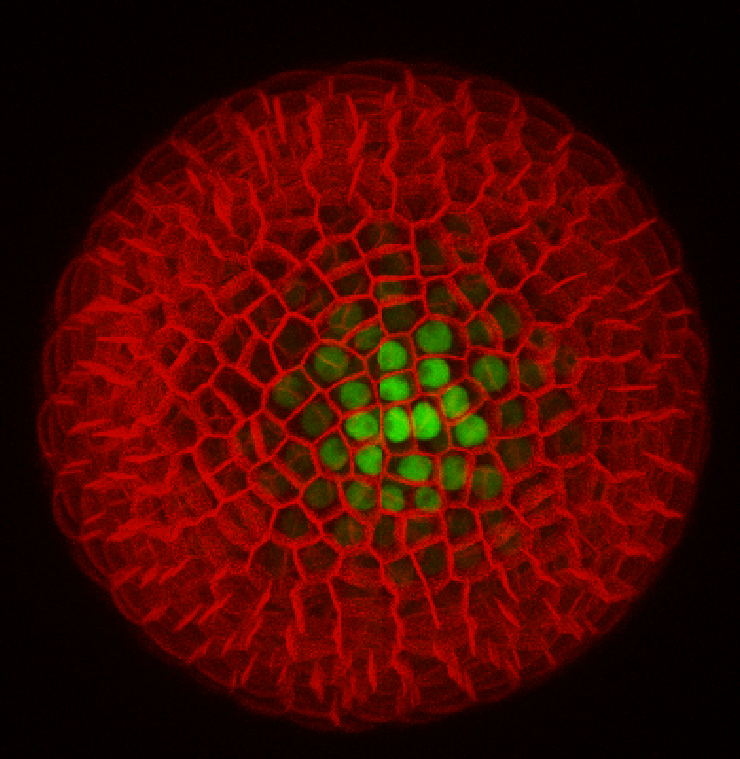
\includegraphics[width=.4\textwidth]{raw_channels.png}
  \caption[Confocal microscopy data]{Top view of raw data as produced by the
    confocal imaging, taken from plant 2 at timepoint 0 hours. In red can be
    seen the membrane channel, merged with the
    nuclear response in green. The nuclear vacuole is observable as shaded dots
    in the green channel. Note also how the L2 and L3 produce a perceived
    fuzziness in the peripheral regions.}
  \label{fig:rawdata}
\end{figure}

\section[Processed image data]{Image pre-processing and segmentation}
In order to eliminate segmentation errors, the ImageJ~\cite{abramoff2004image}
plugin StackReg~\cite{thevenaz1998pyramid} was used
to perform a translation transformation for each stack. Individual slices which
contained horizontal shifts because of vibrations or other types of system
disturbances were identified and replaced with the nearest slice that contained
no such shift. The z-directional stretching due to stem elongation was corrected for by mapping
the low-resolution stacks to the high-resolution ones in order to attain
stretching factors that the images were thereafter corrected for. 

For the membrane channel, noise removal was done by Gaussian and alternative-sequential
filtering. The filtered z-stacks were then watershed in 3D using the
algorithm implemented in the segmentation software MARS-ALT (see
\cref{sec:marsalt}). Segmentation and
tracking were thereafter performed using the same software. Cellular volumes
were calculated as the sum of voxel volumes belonging to the same cell.
The tracking, also performed using MARS-ALT, was assessed for quality using an F1
score between the parent and corresponding daughter cell. For all analyses
discussed in this report, a cutoff value of 0.30 was set for the tracking in
order to account for incorrect mappings. These cells are included in the
overall analysis, but excluded from all cell line related investigations.
A longer outline of errors and exceptions in the segmentation is presented in
\cref{sec:data_errors}.   

The nuclear and membrane data were deconvolved to account for the microscope's point-spread
function using the \textit{PSF distiller} tool from Huygens software
15.05~\cite{ponti2007huygens}. As
in the membrane case, the nuclear channels were adjusted with the  
corresponding stretching factors and thereafter segmented using segmentation
tool Costanza~\cite{costanza} (see \cref{sec:costanza}). Whenever we in this
thesis mention the CLV3 expression, we refer to the mean fluorescence of the
voxels belonging to the corresponding nucleus. 

\begin{figure}[H]
    \centering
    \begin{minipage}{0.49\textwidth}
        \centering
        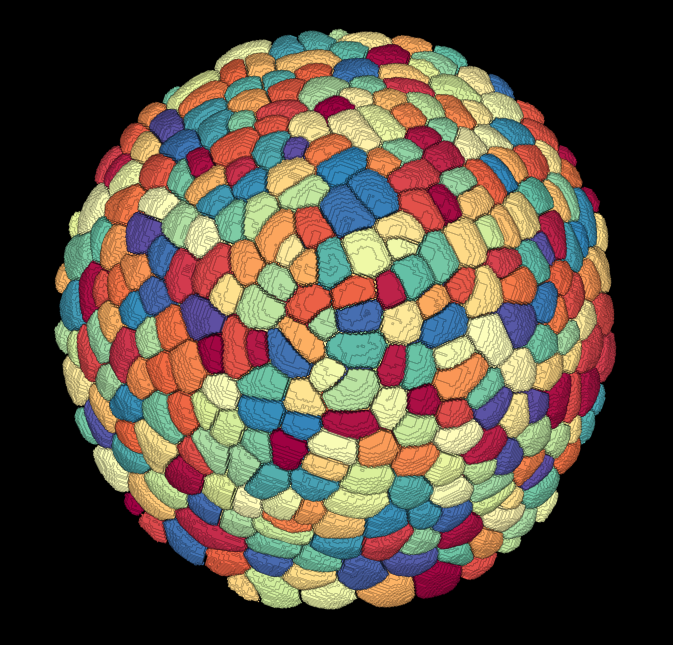
\includegraphics[width=.95\textwidth]{plant18_t0.png}
      \end{minipage}\hfill
      \begin{minipage}{.49\textwidth}
        \centering
        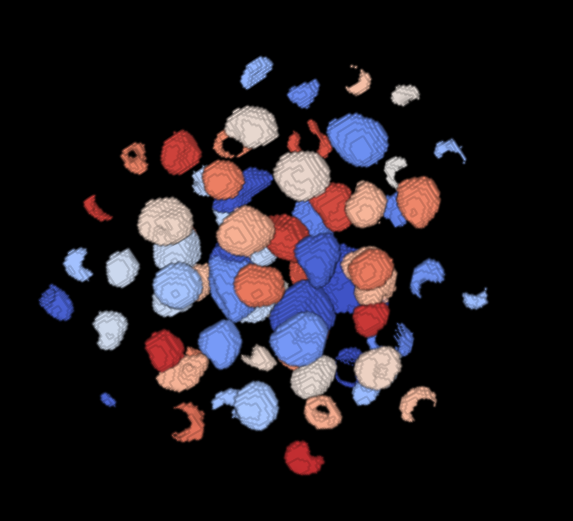
\includegraphics[width=\textwidth]{plant18_t0_n.png}
      \end{minipage}
      \caption[Segmented data]{Segmented membrane and nuclear channels as output by
        visualisation software TissueViewer after MARS-ALT and
        Costanza segmentation respectively (see \cref{sec:software_descr}). Note in the nuclear channel
        how the loss of signal due to the vacuole causes miss-segmentation in
        multiple cases. Figures taken from plant 18, timepoint 0 hours. Nuclear
        and membrane channels not on same scale.}  
\end{figure}

% Nuclear and membrane mapping
Due to the membrane and nuclear segmentations originating from different
softwares, a separate mapping step was required in order to relate nuclei to
their corresponding cell membranes. This was done by taking the centroid spatial
coordinates, as defined by the basins of attraction acquired during
segmentation, of all respective segmented items, and mapping them using a
least-squares approach. Duplicately mapping nuclei were then
consolidated as described in \cref{sec:filtering}. 

% Distance measures (d2t / circ)
Measures of distances to the apex were done in multiple ways. The four methods
herein considered consist of a definition of the tip based on 1) the spatial
coordinates, 2) the expression value, 3) expression-weighted spatial
coordinates, and 4) a least-square fit of a paraboloid to raw meristem images.
For the paraboloid fit, this was done by taking the top 75 images part of the
confocal z-stack, in order to minimise the fitting impact of primordia that
are more prominent in the deeper levels.
In the case of spatial coordinates, the average $x-y$  
coordinates of $n$ nuclei were chosen, complemented with the highest $z$ value
registered in the corresponding timeframe. For the second case, the apex was
defined as the mean spatial coordinates of the $n$ highest expressing CLV3
nuclei. The weighted apices were similarly determined through transformation via
$\bar{x}_{w} = \sum^{n}_{i} \bar{x}_{i}I_i / \sum_{i} I_i$, where $n$ again denotes number of cells included,
arranged by highest z-value, and $I$ the CLV3 intensity for the
corresponding cell.
Lastly, the paraboloid fit to the meristem was used to define the apex by
taking the coordinates of the region have a zero-valued derivative. For both the
segmentation-dependent approaches, the data was set to exclude subepidermal
layers in order to prevent biases. For most of our measures relating to a
definition of the apex in this thesis, we refer to the top as the one defined by
the four highest expressing cells, unless otherwise stated.

To achieve a cell-resolution description of distances in the SAM,
an auxiliary measure of cell distances was used in the form of a cell-wise
grouping. In the cell value utilising definitions of the apex above, cells
included in the definition were set to have a cell-wise distance of 0. The
neighbours of these cells were in turn defined to have a distance value of 1,
and so on recursively. Again, we exclude the plants lacking nuclear data from
measures utilising this, as described in \cref{sec:missingtp}. In addition,
whenever cells deeper in the tissue than L2 are  
referenced, we refer to these as L3 and L3$+$ interchangeably.

\section[Data processing]{Data processing}
\label{sec:data_processing}

\subsection[Data analysis tools]{Development of a data analysis pipeline}
\label{sec:pipeline}
Data was analysed predominantly using R through the development of a single
modular pipeline, denoted \textit{extractoR}. This was designed to build 
primarily on a sequential software design pattern,  
incorporating parallelisation and batch processing for treatment of the multiple
timelapses. A more detailed description is outlined in~\cref{sec:extractoR}.

\subsection[Data filtering]{Data filtering}
\label{sec:filtering}
Due to thresholding effects during the segmentation, some
individual nuclei are occasionally identified as two or more. Nuclei were
therefore mapped to the corresponding cells using a minimum euclidian distance
measure between the respective centroids. The nuclear quantified metrics were
then corrected using the functions found in \cref{tab:consolidation_methods}. In
addition to this, all mentions of numbers of nuclei are with respect to the
number of cells containing at least one nuclear volume identified
within them.

For the data analysis section, data was excluded due to apparent segmentation
errors. This was done for each plant in isolation, with the outline of the
filtering described in \cref{tab:filtering}. The choice of allowed
deviance was done based on the distribution shape, 
with particular consideration 
taken to the nuclear and membrane volumes, where no lower boundary was set. The
maximal neighbour distance was chosen due to the typical lack of data for cells more
than $7$ cell distances from the apex. Lastly, due to division events where
loss of nuclear signal took place, we filter out expression values which are
less than 70~\% of the magnitude in the previous, as well as subsequent, timepoint.

\begin{table}
  \parbox{.47\linewidth}{
    \centering
    \begin{tabular}{ll}                            \toprule
      \textbf{Parameter} & \textbf{Value}       \\ \midrule
      Maximal membrane volume & $\mu + 3\sigma$ \\
      Minimal membrane volume & 0               \\
      Maximal nuclear volume  & $\mu + 5\sigma$ \\
      Minimal nuclear volume  & 0               \\
      Maximal apical distance & $\mu + 3\sigma$ \\
      Maximal neighbour distance & $7$          \\ \bottomrule   
      \vspace{.1em}
    \end{tabular}
    \caption[Filtering settings]{Filtering settings in order to account for outliers in the data.
      Typical causes of these are missegmentation such as the merging of multiple
      nuclear membranes of nuclei. Because the quaility declines with the distance to the
      apex we here limit our analysis to cases where cells are within a distance
      of 7 cells from the defined apex.}
    \label{tab:filtering}
  }
  \hfill
  \parbox{.47\linewidth}{
    \centering
    \begin{tabular}{lc}                                 \\ \toprule
      \textbf{Metric}       & \textbf{Summary function} \\ \midrule
      Coordinates (x, y, z) & mean                      \\
      Nuclear volume        & sum                       \\ 
      Nuclear expression    & mean                      \\ \bottomrule
      \vspace{.1em}
    \end{tabular}
    \caption[Consolidation methods for duplicate nuclei]{Consolidation methods applied for cases where multiple nuclei were
      mapped as belonging to the same membrane cell. This happens mainly due to
      errors  when one nuclei is identified as multiple in the
      binarisation step of the segmentation.}
    \label{tab:consolidation_methods}
  }
\end{table}

\section[Models of Gene Regulatory Networks]{Models of Gene Regulatory Networks}
\label{sec:models_of_grns}
\subsection[Mathematical Formulation]{Mathematical Formulation of Biochemical
  Reactions}
\label{sec:mathematical_form}

\subsubsection[Mass-action Kinetics]{Mass-action Kinetics}
\label{sec:mass_action}
The formulation of processes in GRNs focuses primarily on two aspects: synthesis
and degradation of matter, which usually takes the form of molecular
concentrations or absolute abundance. As outlined in \cref{sec:modelling}, we
here work using an ODE or SDE description of  
our regulatory systems. 

In this study, we represent our molecular reactions using mass-action
interactions and Michaelis-Menten kinetics; both relying on the na\"ive
assumption that our primary reagents here act in isolation of other possibly
intervening molecules. As part of our formalism, we write
\begin{equation}
  S \xrightleftharpoons[k_{f}]{k_{b}} P
  \label{eq:simple_reac}
\end{equation}
to express that some substrate $S$ is turned into a product $P$ by some given
\textit{forward rate constant} $k_f$. Likewise, as the reaction is \textit{reversible}, the
product $P$ is transformed back into $S$ with the \textit{backward rate constant}
$k_b$. 

The \textit{law of mass action} states that the rate of a reaction
is proportional to its affinity, e.g.\ $k_f$, and the concentration of the
reacting species, here $S$. The reaction rate of the production of $P$ would thus be
$r_f = k_f S$. However, the rate of change of reactant $P$ also depends
on the backward affinity, which would give the overall rate-of-change for $P$ as
\begin{equation}
  \Delta P = k_f S - k_b P.
  \label{eq:mass_action_noninf}
\end{equation}
In the infinitesimal limit, we analogously have 
\begin{equation}
  \frac{\dd P}{\dd t} = k_f S - k_b P,
  \label{eq:mass_action_inf}
\end{equation}
i.e.\ on the form of a differential equation, which will be the baseline for our
formulations. Similar to the formulation of a rate-of-change of $P$, we can do the
same for species $S$, and our system is then fully represented as a system of
differential equations.

Expanding on this, we can easily solve for the steady-state concentrations of
the system by assuming that all rates average to zero. In our example above, this
gives us 
\begin{equation}
  \frac{k_f}{k_b} = \frac{P}{S},
  \label{eq:mass_action_ss}
\end{equation}
which holds in general, regardless of the number of reacting
species~\cite{horn1972general}.

\subsubsection[Michaelis-Menten Kinetics]{Michaelis-Menten Kinetics}
\label{sec:mm}
A conceptual drawback of the mass-kinetics formulation is the possibility to
have infinite reaction rates, whereas the molecular reactions in nature typically
are restricted by some means. One way to account for this is through
\textit{Michaelis-Menten kinetics}, which describes enzymatic chemical
reactions. In these, the trivial example introduced in \cref{eq:simple_reac} is
expanded to include an enzymatic agent such that
\begin{equation}
  E + S \xrightleftharpoons[k_f]{k_b} ES \xrightarrow{k_p} E + P.
  \label{eq:enzymatic_react}
\end{equation}
In other words, an enzyme-like molecule binds to the substrate $S$ such that the
complex $ES$ is formed. This complex is thereafter transformed into the product
molecule $P$ and again the enzyme $E$. Assuming a total enzyme concentration of
$E_{tot}$ and the assumption that the enzyme-substrate binding process is in
equilibrium, the rate-of-change of the product can be rephrased to be on the
form 
\begin{equation}
  \frac{\dd P}{\dd t} = V_{max} \frac{S}{K + S},
  \label{eq:michaelis-menten}
\end{equation}
where $K = K_f / K_b$ and $V_{max} = k_pE_{tot}$. This expression is said to be
on \textit{Michaelis-Menten} form, where $V_{max}$ is the maximal
activation rate of the protein, and $K$ can be thought of as a saturation
coefficient.

Extrapolating on this type of reaction, introducing $n$ enzymatically acting
molecules instad gives the standard \textit{Hill equation} form, namely
\begin{align}
  \frac{\dd P}{\dd t} &= V_{max} \frac{S^n}{K^n + S^n},\hspace{.8em} \text{and} \\
  \frac{\dd P}{\dd t} &= V_{max} \frac{K^n}{K^n + S^n}
  \label{eq:hill}
\end{align}
for an activating and repressing reaction respectively~\cite{chou1977simple}.

\subsection[Stochastic Simulations]{Numerically solving stochastic systems}
\label{sec:stoch_sim}
\subsubsection{Gillespie Algorithm}
\label{sec:gillespie}
The Gillespie algorithm is a discrete approach for simulating stochastic
molecular dynamics. It first appeared in print by Dan Gillespie in
1977~\cite{gillespie1977exact}, and has
since been widely used for stochastic simulations in multiple fields.

While being computationally expensive, the Gillespie algorithm compensates for
its lack in tractability by producing a statistically exact trace of the
molecular dynamics of a system. 

The algorithm originates in the formulation of the \textit{chemical master equation},
which specifies the rate of change of the transition probability between states
in the form of 
\begin{equation}
  \dfrac{\partial P\left( x,t | x_0, t_0 \right)}{\partial t} = 
  \sum_{j =
    1}^{M} \left[ a_j\left( x-v_j \right)P\left( x-v_j, t|x_0,t_0 \right) -
    a_j(x)P\left( x,t|x_0,t_0 \right) \right]
\end{equation}
where $a$ defines the reaction probability, or propensity, for each type of
reaction ($j \in {1, \ldots, M}$), and
$v$ the stoichiometry, i.e. information of how the molecular species are changed
due to the reaction. $P(x,t | x_0, t_0)$ on its own denotes the probability of
$X(t) = x$, given that the initial value is $x_0$. Solving the master equation
analytically is usually complicated, so  
simulating a complex biological system using the Gillespie approach can often be
far more tractable.

Procedurally, the algorithm can be formulated in four steps: 
\begin{description}
  \item[Initialisation] Generation of number of molecules and reaction
    parameters. 
  \item[Randomisation] Generation of random numbers to determine 1) next
    interaction, and 2) the time increment.
  \item[System update] Time and molecular numbers are update correspondingly
    to the determined event in step 2.
  \item[Repetition] Step 2-4 are repeated until some stop condition is met.
\end{description}

In principle, the Gillespie algorithm is calculating two variables determining
1) when the next reaction happens, and 2) which the next reaction is.
The time until the next reaction at time $t$ is denoted $\tau$ and can be shown
to be an exponential distribution centered  
at $1 / \sum_{j=1}^{M}a_j(x)$ for some molecular concentration $x$, i.e.
\begin{equation}
  p(\tau = t') = \sum_{j=1}^M a_j(x)e^{-\sum_{j=1}^M a_j(x)t'}
  \label{eq:gill:time}
\end{equation}
with the reaction probability instead being described by the normalised
propensity. Historically, due to the limitation of random number generators, the
time update has been described as being drawn from 
\begin{equation} 
  \displaystyle
  \tau = \dfrac{1}{\sum_{j=1}^M a_j(x)} \ln\dfrac{1}{r_1}
  \label{eq:gill_time_update}
\end{equation}
with $r_1$ denoting a uniformly distribution random number in the interval
$(0,1]$.

\subsubsection{Milstein's Method}
\label{sec:milstein}
If there is no requirement for exactness, less computationally intensive
alternatives to Gillespie's algorithm exists. One such example is the
\textit{Langevin} formulation of chemical systems, which utilises SDEs to
attain an approximate solution to the system trajectory, and is particularly
useful when the number of molecular reagents is high. 

The Langevin formulation, like Gillespie's, utilises the chemical master
equation to compute the behaviour of the system. In principle, the Langevin
formulation can be said to reformulate a deterministic increment of the form
\begin{equation}
  X_i(t + \dd{t}) = X_{i}(t) + \sum_{j=1}^M
  v_{ji}a_j(X(t))\dd{t}
  \label{eq:deterministic}
\end{equation}
to the stochastic form
\begin{equation}
  X_i(t + \dd{t}) = X_{i}(t) + \sum_{j=1}^M
  v_{ji}a_j(X(t))\dd{t} + \sum_{j=1}^M
  v_{ji}a_j^{1/2}N_j(t)\dd{t}^{1/2}
  \label{eq:stoch}
\end{equation}
where $X$ denotes the molecular number, $v$ the stoichiometric coefficient of the
reaction in question, and $N_j$ are temporally uncorrelated and statistically
independent, Gaussian random numbers with mean 0. From this stage, the equation
is then easily extended to its multivariate form, namely
\begin{equation}
  X_i(t + \dd{t}) = \sum_{j=1}^Mv_{ji}a_j(\bar x) \dd{t} +
  \sum_{j=1}^M v_{ji}{a_j}^{1/2}(\bar x) N_j(t) \left( \dd t \right)^{1/2}
  \label{eq:stoch_multi}
\end{equation}

Milstein's approach to solving this equation numerically utilises
\cref{eq:stoch} on the differential form 
\begin{equation}
  \dd X_t = a(X_t) + b(X_t) \dd W_t
  \label{eq:milstein_form}
\end{equation}
where $W_t$ is a continuous-time stochastic process. The simulation interval
$\left[ t_0, T \right]$is then partitioned into parts of size $\Delta t = T /
N$, where $N$ is the number of partitions. We thereafter define the update
\begin{align}
  Y_{n+1} &= Y_n + 
  a(Y_n)\Delta t + 
  b(Y_n)\Delta W_n +
  \dfrac{1}{2}b(Y_n)b'(Y_n)\left( \left( \Delta W_n \right)^2 - \Delta t \right) \\
  Y_{n+1} &= Y_n + 
  a(Y_n)\Delta t + 
  b(Y_n)\Delta W_n + 
  \dfrac{1}{2} b(Y_n)b'(Y_n) \left(\Delta W_n\right)^2 
  \label{eq:milstein_deriv}
\end{align}
on It\={o} and Stratonovich form respectively. Here $b'$ denotes the spatial
derivative of $b$, whereas $\Delta W_n = W_{\tau_{n+1}} - W_{\tau_n}$. The
difference between the It\={o} and Stratonovich form in turn is the
interpretation of the integral of $\dd W_t$~\cite{klimontovich1990ito}. In many cases, it is
preferable to express the numerical update on a derivative-free form, which can
be done through a Runge-Kutta like approach~\cite{garcia2011comparison} in order to state the final,
multivariate expression as 
\begin{equation}
  Y_{i, n+1} = Y_{i, n} + a_i\left( Y_{i,n} \right) \Delta t + 
  b_{ii}(Y_{i,n}) \sqrt{\Delta t} N_i + \dfrac{1}{2\sqrt{\Delta t}} \left[
    b_{ii}(\bar x, n) - b_{ii} \right]
  \Delta t (N_i)^2 
  \label{eq:milstein_deriv_free}
\end{equation}
where a supporting predictory step is calculated in the form of 
\begin{equation}
  \bar {x_i} = x_i + a_i\left( Y_n \right)\Delta t + b_{ii}\sqrt {\Delta t}.
  \label{eq:milstein_predictor}
\end{equation}
Algorithmically, the Milstein approach is of strong order of convergence
$\mathcal O \left( \sqrt{\Delta t }\right)$ and weak order $\mathcal O \left(
  \Delta t \right)$~\cite{garcia2011comparison}. In this thesis, we utilise the Milstein approach under the
Stratonovich interpretation.

\section{Network modelling approach}
\label{sec:modelling_approach}
In this thesis, we model regulation of gene expression using Hill equations for
production and exponential decay for degradation. Gene products are instead
set to undergo linear production with respect to the activating gene, as well as
diffusion. As for gene expression, proteins are modelled using exponential
decay. In total, the equations governing the regulation for a gene $X$ and its
protein $x$ can then be formulated as

\begin{align}
  \frac{\dd X}{\dd t} &= 
  \prod_{a=1} V_{max}\frac{X_a^{n_{a}}}{K_a^{n_a} + X_a^{n_a}}
  \prod_{r=1} \frac{K_r^{n_{r}}}{K_r^{n_r} + X_r^{n_r}} -
  dX, \ \ \ \text{and} \\
  \frac{\dd x}{\dd t} &= pX + D\Delta x - dx,
  \label{eq:gene_expr_reg}
\end{align}
where $\Delta$ is the Laplace operator. In a deterministic framework, the steady
state of the system can then be solved algebraically if the
parameters of the system are known. In this thesis, whenever we simulate our
stochastic networks, we first compute the steady state of the system using this approach.

The two models we herein consider consist of 1) simple, enzymatic WUS actvation
of CLV3, and 2) the former with multiplicative L1 activation. That, is our
activation of CLV3 can in the two models be described by the equations 

\begin{align}
  \frac{\dd C}{\dd t} &= v_{max} \frac{w^n}{K^n + w^n} - dC, \ \ \
  \text{and} \\
  \frac{\dd C}{\dd t} &= v_{max} 
  \frac{w^{n_{w}}}{K_{w}^{n_{w}} + w^{n_{w}}} 
   \frac{L1^n}{K_{L1}^{n_{L1}} + L1^{n_{L1}}} - dC
  \label{eq:model_eqs}
\end{align}

respectively. For our simulations, we use Gillespie to simulate the former, and
transition into Langevin formalism in the latter case due to the increase in
system size. Parameter sets used can be found in \cref{sec:modelparams}. The
spatial structure of the model in both cases consist of a 1D line of cells
undergoing diffusion with their nearest neighbours. WUS activation is located to
a single leftmost cell, denoting the apex, whereas the rightmost end contains a
``sink'' molecule, through which molecules in interaction with can diffuse out of
the system.



%!TEX root = ../thesis.tex
%*******************************************************************************
%****************************** Third Chapter **********************************
%*******************************************************************************

\chapter{Results}

% **************************** Define Graphics Path **************************
\ifpdf
    \graphicspath{{Chapter3/Figs/Raster/}{Chapter3/Figs/PDF/}{Chapter3/Figs/}}
\else
    \graphicspath{{Chapter3/Figs/Vector/}{Chapter3/Figs/}}
\fi

% Oscillations 
\section{Regulation of the CLV3 domain induces periodicity when perturbed}
When tracking the number of CLV3 nuclei identified by Costanza, the results
observable in \cref{fig:clv3_trajs} shows the number of observed CLV3 nuclei
increasing for plants 2, 4, 13, and 15, corresponding to a visually observable
enlargement of the CLV3 domain in \FIG (timelapse of example plant over 4
timepoints?). Similarly, fluctuations in this number can be seen not to 
correlate with the mean expression as described in
\cref{tab:corr_nNucl_meanExpr}. % and therefore ought to be structural

\begin{figure}[H]
  \centering
  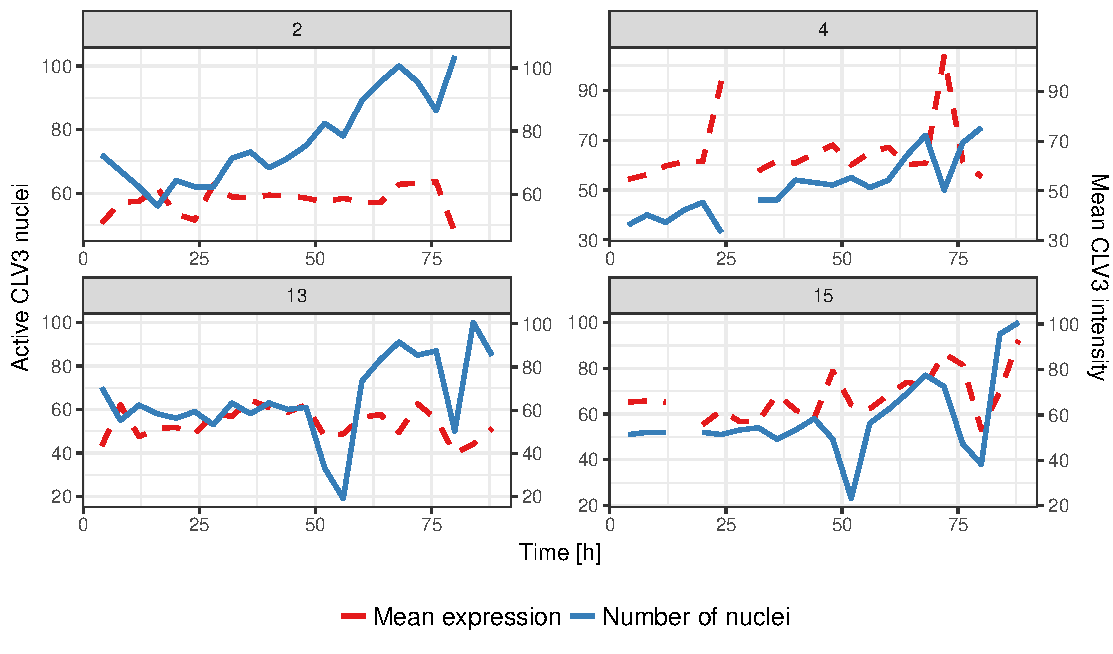
\includegraphics[width=.8\textwidth]{nNucl_trajectories.pdf}
  \caption{Add caption}
  \label{fig:clv3_trajs}
\end{figure}

\begin{table}
  \centering
  \caption{TODO}
  \label{tab:corr_nNucl_meanExpr}
  \begin{tabular}{ll}  \toprule
    Plant & p-value \\ \midrule
    2     & 0.48    \\
    4     & 0.84    \\
    13    & 0.91    \\
    15    & 0.11    \\ \midrule
    All   & 0.50    \\ \bottomrule
  \end{tabular}
\end{table}

In order to assess the extent of the fluctuations the lines were detrended using
a second order Loess fit to each curve. When performing a continuous time
Fourier transform in order to extract amplified modes, the plants have are
biased towards the fourth mode in each respective transformation, as depicted in
\cref{fig:modes}, which corresponds to periodicity of $\sim$16~hours. 

\begin{figure}[H]
  \centering
  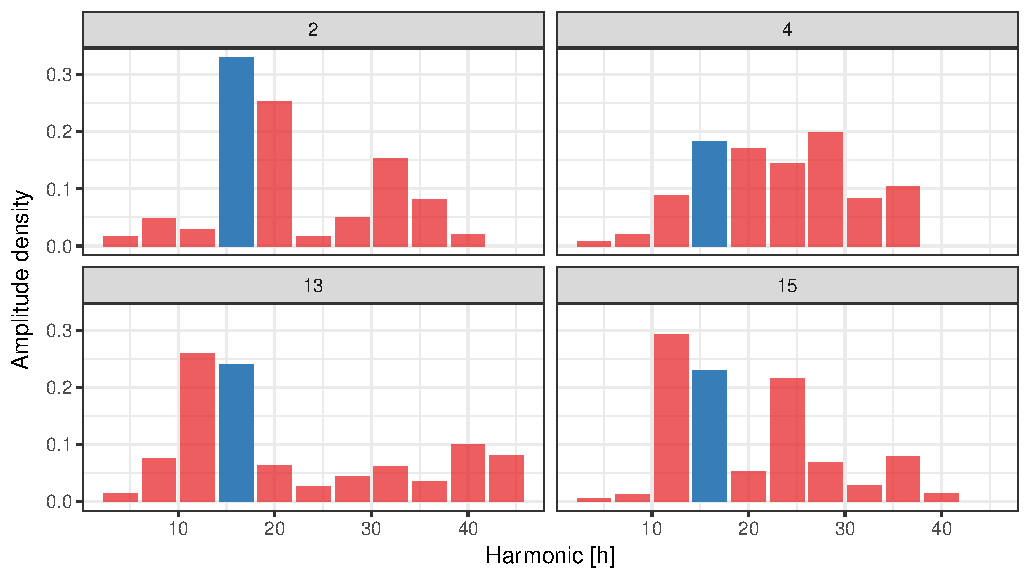
\includegraphics[width=.7\textwidth]{periodogram.pdf}
  \caption{Add caption}
  \label{fig:periodogram}
\end{figure}

\todo{map this to light / dark hour cycles?}
% and are hence not circadian

In addition to this periodicity, the number of nuclei identified correlates
positively with the number of division events observed in each timepoint for
three out of the four plants (\cref{fig:corr_nNucl_nDivs}). Plant 13, like in 
\cref{fig:clv3_trajs} is the only anomously behaving specimen.
\unsure{Should I add other correlations and just draw plots?}

\begin{figure}[H]
  \centering
  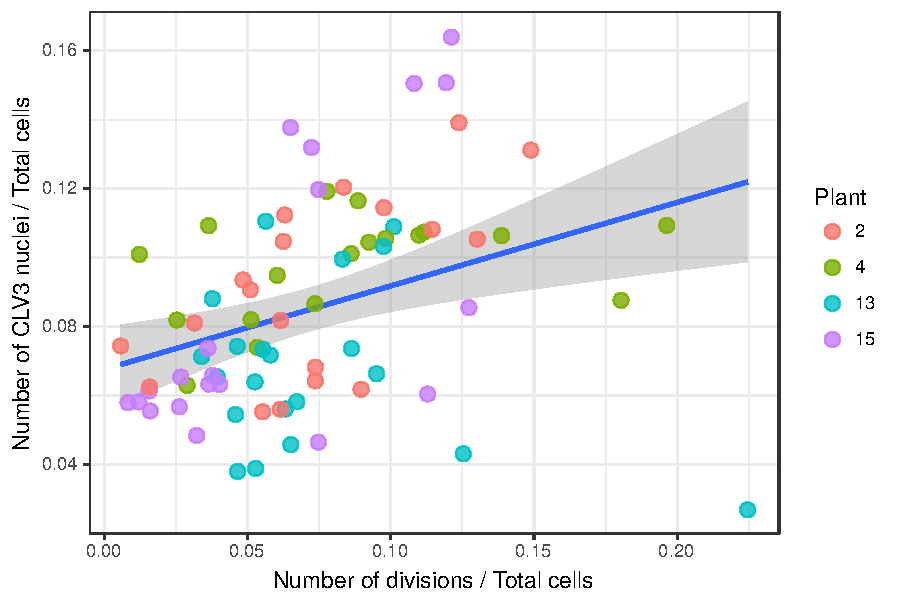
\includegraphics[width=.7\textwidth]{corr_nNucl_nDivs.pdf}
  \caption{Add caption}
  \label{fig:corr_nNucl_nDivs}
\end{figure}

\section{CLV3 noise is kept at bay at apex}

Variance in the expression of CLV3 is suppressed in the apical cells, as can be
seen in \cref{fig:expr_vs_d2t}. This appears true for all plants, although plant
in particular shows tendencies of having a few lowly expressing apical cells at
several timepoints. It should however be noted that it is possible that errors
in the tracking produces this type of data. Accounting for this possibility, all
plants have hysteresis-like shapes. Nevertheless, the distribution of expression
values at distinct distances does not appear to be bimodal, as would indicate
bistability in stem cell regulation. Instead, the data suggests an apparent CLV3
gradient, proportional to the distance to the apex more in radial terms than
in bimodal. 

Using a simple model replicating the epidermis, we are possible to replicate the
shape of the distribution assuming enzymatic CLV3 activation by a WUS gradient
(\cref{}). The enzymatic activation is in this formulation necessary in order to
attain the sigmoidal shape of the curve, where the extent of noise ultimately
depends on tha abundance of the WUS protein.
\FIG

\begin{figure}[H]
  \centering
  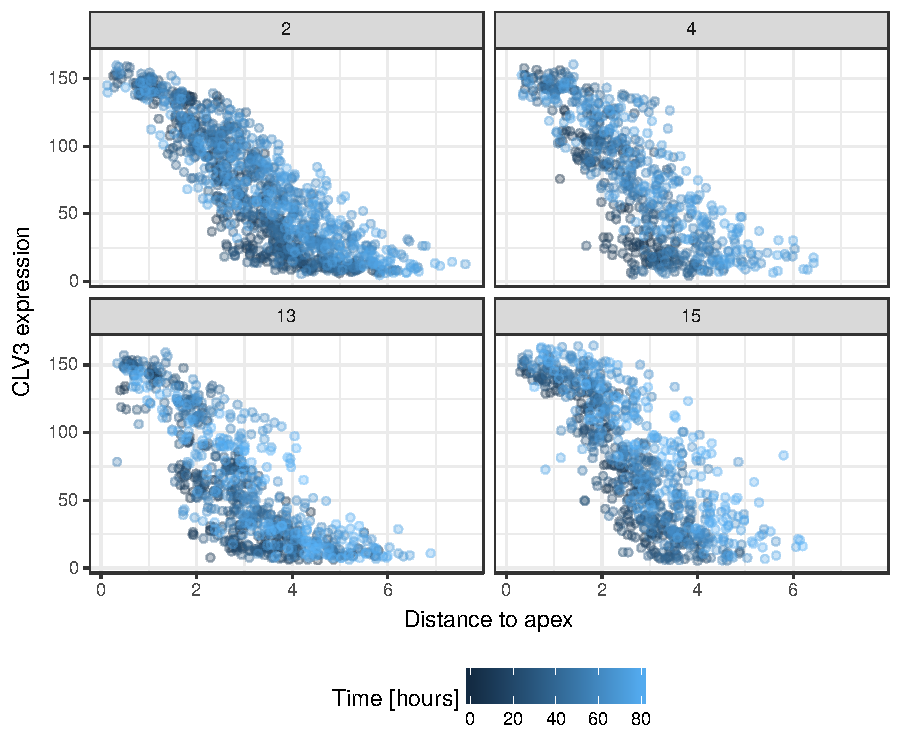
\includegraphics[width=.8\textwidth]{clv3_vs_d2t.pdf}
  \caption{Add caption}
  \label{fig:clv3d2t}
\end{figure}

A layer-wise separation of the CLV3 expression can be seen in particular between
L1 and L2, as visualised in \cref{fig:epireg}. In L1, the correlation between
CLV3 expression and nuclear volume appears sigmoidal, although consideration
should be taken to the fluorescence ceiling due to the laser. In contrast, both
L2 and L3 have linear relationships, indicating the possibility of epidermal
activation alternatively subepidermal repression altering the distributions.
Also in the distributions of CLV3 expression in relation to the distance to the
apex this effect is observable.



\begin{figure}[H]
  \centering
  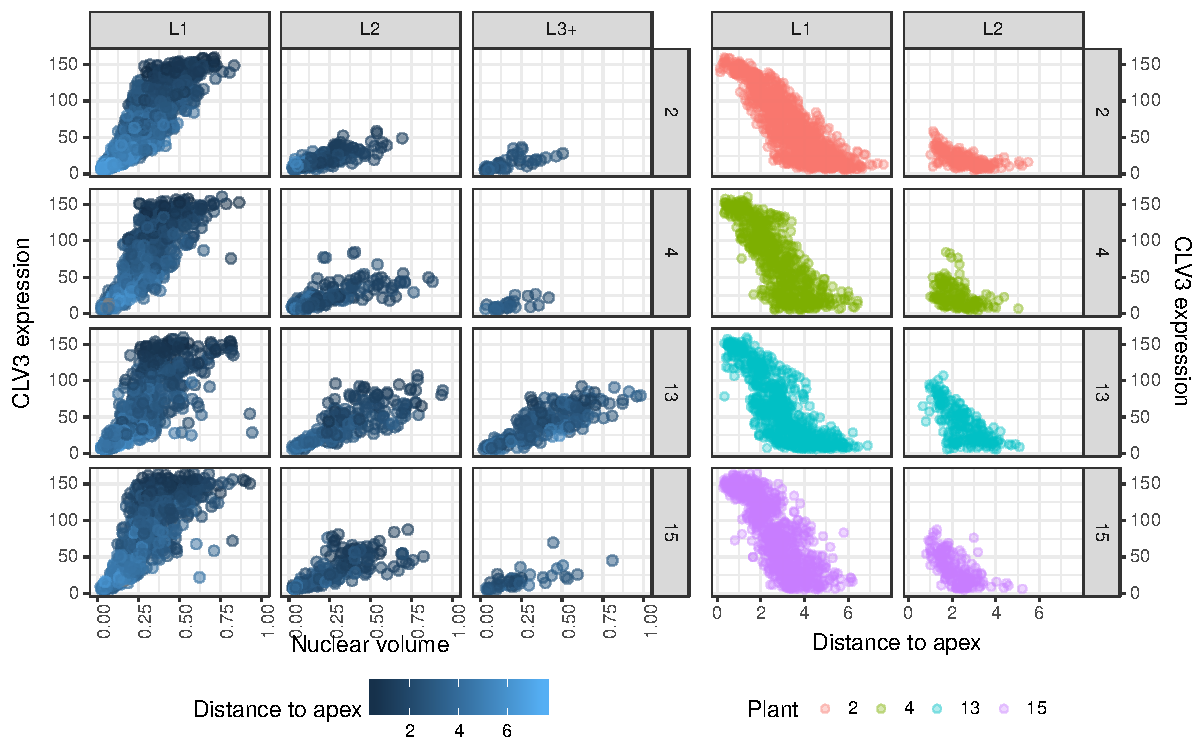
\includegraphics[width=\textwidth]{epireg.pdf}
  \caption{Add caption}
  \label{fig:epireg}
\end{figure}

%\section{Distribution shifting suggests epidermal regulation}
%\subsection{CLV3 is induced in the epidermis}




 % This holds regardless of what distribution looks like

 \section{Functional clustering implies dsRED technical artefacts}

 \begin{figure}[H]
   \centering
   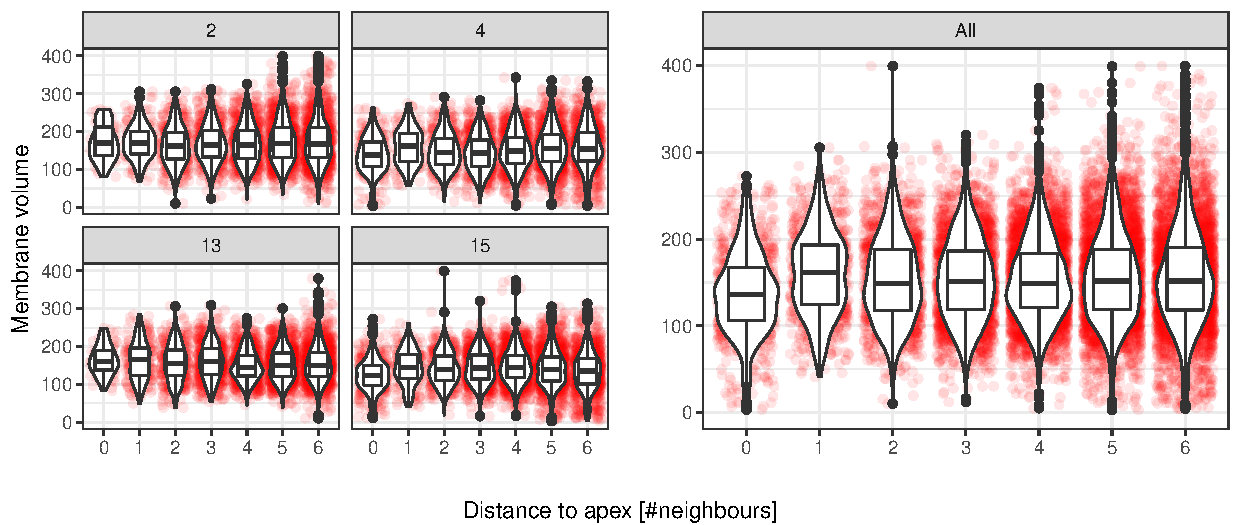
\includegraphics[width=\textwidth]{mvol_apex.pdf}
  \caption{Add caption}
  \label{fig:mvol_apex}
\end{figure}

\begin{figure}[H]
   \centering
   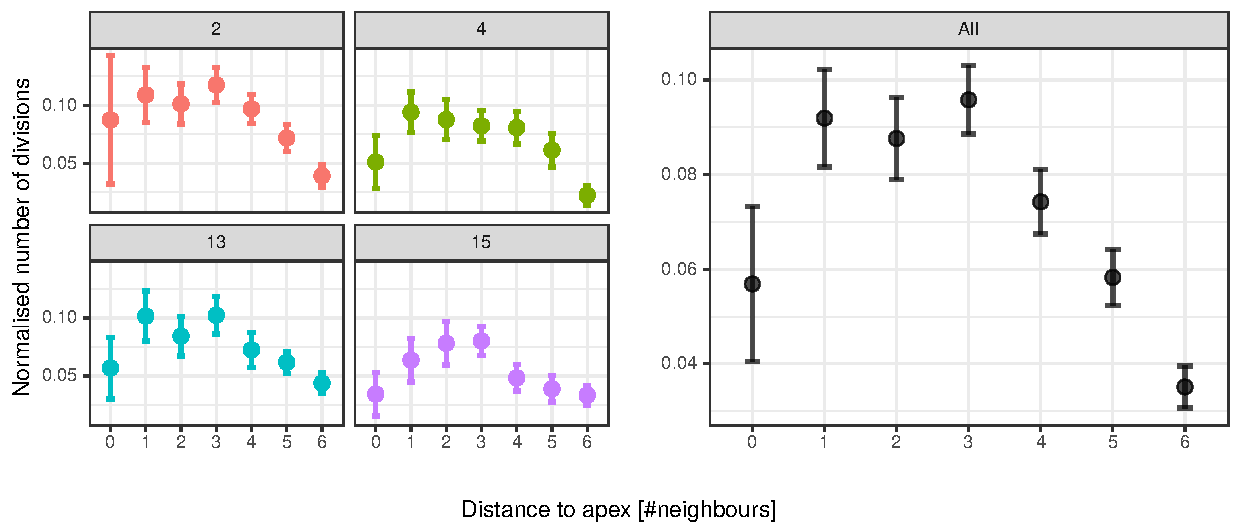
\includegraphics[width=\textwidth]{nDivs_apex.pdf}
   \caption{Add caption}
  \label{fig:mvol_apex}
\end{figure}


\begin{figure}[H]
  \centering
  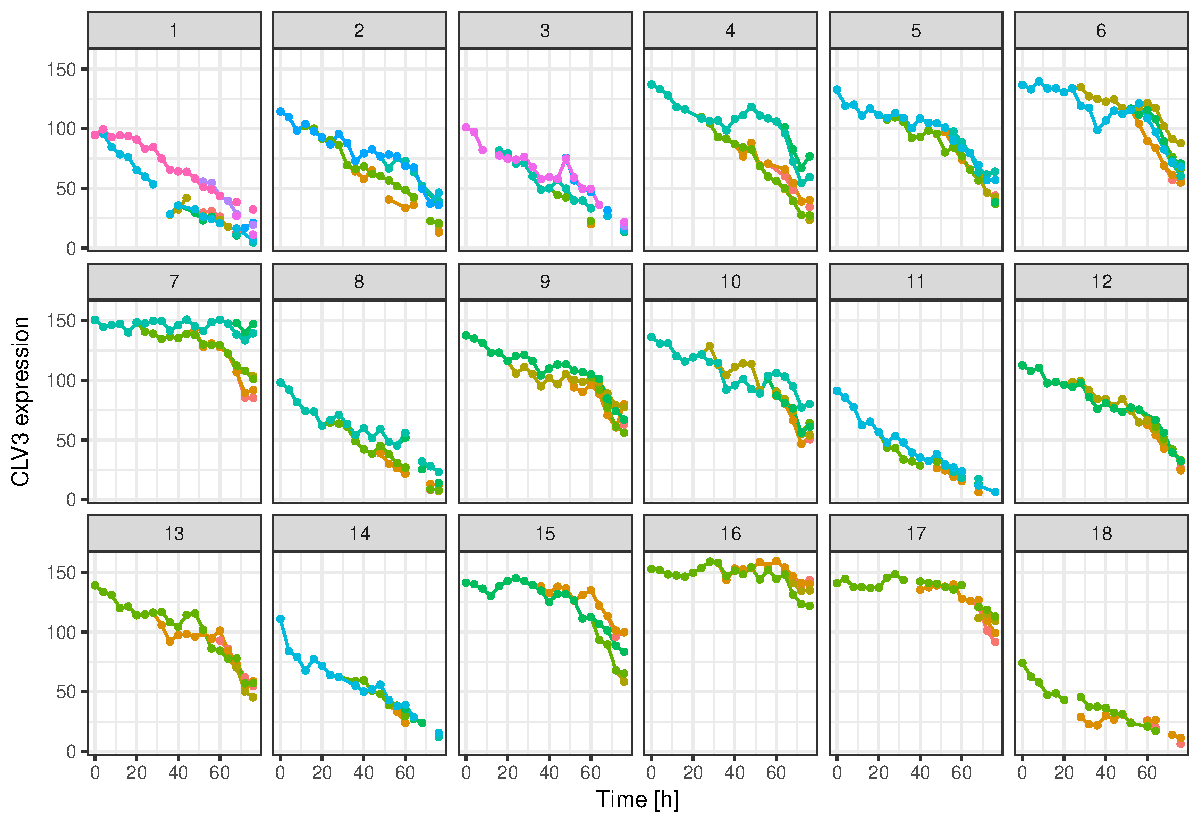
\includegraphics[width=\textwidth]{plant2_trajectories.pdf}
  \caption{Add caption}
  \label{fig:corr_nNucl_nDivs}
\end{figure}

\begin{figure}[H]
  \centering
  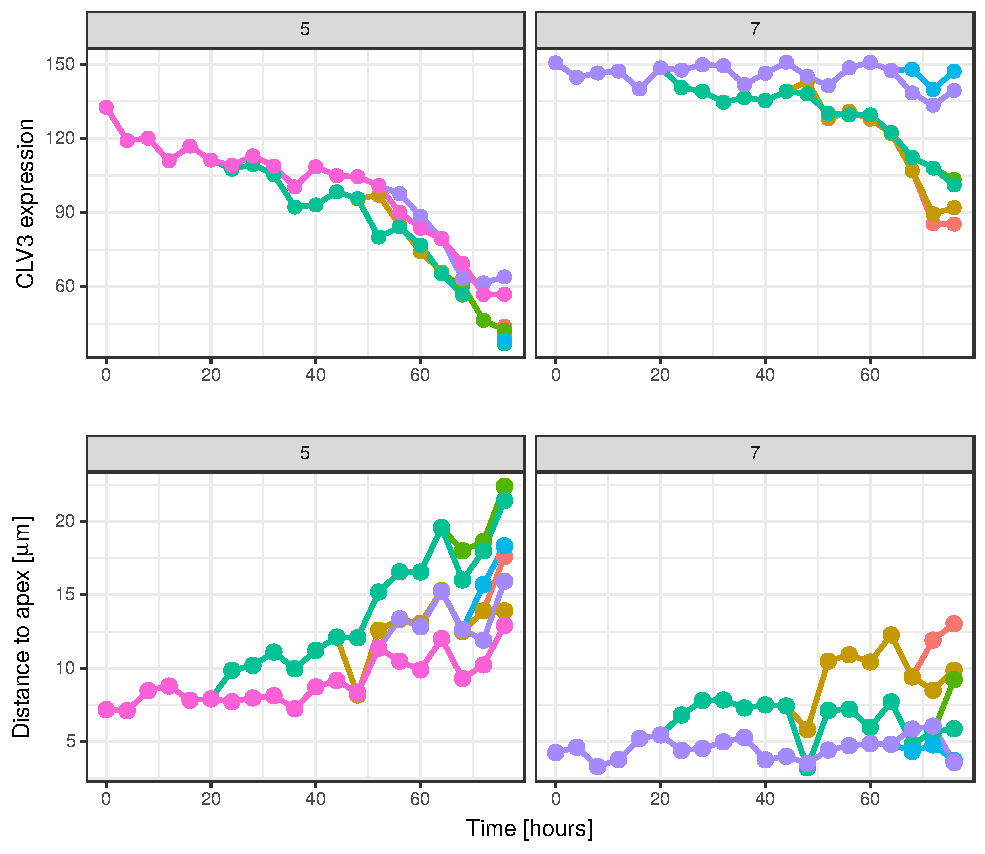
\includegraphics[width=.5\textwidth]{select_trajectories.pdf}
  \caption{Add caption. }
  \label{fig:select_trajs}
\end{figure}

\begin{figure}[H]
  \centering
  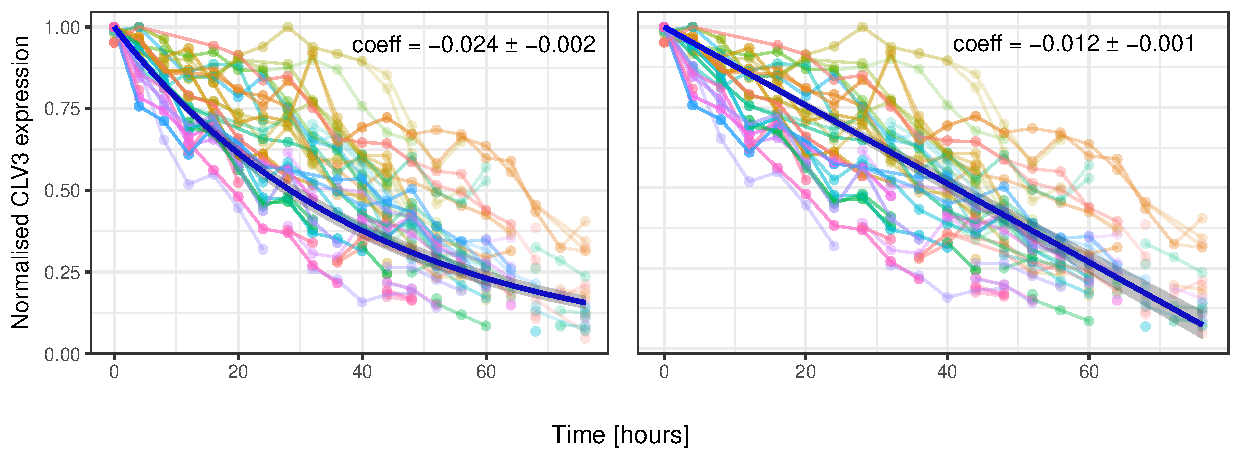
\includegraphics[width=\textwidth]{dsred_plant2.pdf}
  \caption{Add caption}
  \label{fig:dsred_decay}
\end{figure}

TODO: Justification for decay. Assume movement out of CZ proportional to
division rate $k_{div}$, such that $\dot{R} \propto k_{div}$. We thus have
$R = kt$. Assume linear degradation of CLV3 such that $\dot{C} = -k_{deg} =
\frac{\dd C}{\dd t} = \frac{\dd C}{\dd R} \frac{\dd R}{\dd t}$. We therefore have
$\frac{\dd C}{\dd R} = \frac{\dd C}{\dd t} = -\frac{k_{deg}}{k_{div}}$. Justify
decay rate observed in trajectories or smth like that?


\section{Deep-tissue cells divide at a slower rate}
Still unknown.

%%!TEX root = ../thesis.tex
%*******************************************************************************
%****************************** Third Chapter **********************************
%*******************************************************************************
\chapter{Discussion}

% **************************** Define Graphics Path **************************
\ifpdf
\graphicspath{{Chapter4/Figs/Raster/}{Chapter4/Figs/PDF/}{Chapter4/Figs/}}
\else
\graphicspath{{Chapter4/Figs/Vector/}{Chapter4/Figs/}}
\fi

\section{NPA dilution induces oscillations}
Henrik makes it sound like we actually see oscillations? Might be better to be a
bit conservative here. 

\section{\textit{In vivo} tracking of apical stem cells agrees with hypothesis}

\section{Distributional cues give hints at regulatory scheme}
\subsection{Activation of CLV3}
Might be a good place to discuss errors and why we don't see stem cells in L2.

\subsection{Longevity (Don't know what this shows yet)}
Spatial cues from division data

\subsection{Defnition of center}
Peak intensity in CLV3 follows general direction of growth? Reasons to doubt
this?

%%!TEX root = ../thesis.tex
%*******************************************************************************
%****************************** Third Chapter **********************************
%*******************************************************************************
\chapter{Outlook}

% **************************** Define Graphics Path **************************
\ifpdf
\graphicspath{{Chapter5/Figs/Raster/}{Chapter5/Figs/PDF/}{Chapter5/Figs/}}
\else
\graphicspath{{Chapter5/Figs/Vector/}{Chapter5/Figs/}}
\fi

\section{Significance of results}
% Few single cells at apex maintained
Our analysis presented herein has given extensive novel insights into the dynamics of
the stem cell niche of AT. In particular, we have showed how the SAM appears to
maintain a few single cells that are truly expressing CLV3, and thus also set
the grounds for further investigations into the variance in and extent of this small
pool of cells; for example, questions we have not addressed herein are the
variability in the size of the true CLV3 domain in relationship to the overall
size and eccentricity of the SAM itself. 

% Dynamic perspective
While previous research has primarily focused on the static view of the stem
cell niche, we have here provided parts also of the dynamic perspective --
something which has previously been severely lacking. Because of this, we are
able to better support the hypothesis of epidermal regulation in the
CZ, and also pointed at cues of the extent of differentiation driving peripheral
signals. That is, our observed differences in functional behaviour for cells at
various distances from the CZ suggests a possible domain for where peripheral
signalling is either present, or simply begins to affect cell functionality.
Using this information can be of use in particular for modelling, where
understanding the extent of unknown regulatory mechanisms can aid in unraveling
their nature.

% 
We have also shown how the CLV3 apex does not coincide with the geometrical
apex, which might have an impact on anisotropic growth and phyllotaxis. This is
a completely unprecedented result, which might provide future insights into how
the interplay is orchestrated between the CZ and the peripheral regions which
undergo primordia initiation.

\section{Expansion of modelling framework}
Our models herein have taken an abstract approach, which while sufficient for
our purposes does not capture the complexity and intricacies of the real tissue.
Modern software tools are now able to generate contact maps from confocal
images, thus creating the means for accurately comparing model simulations to
the real tissue. This is a possible extension to the work herein, which would
also be a natural future validation step. 

Establishing models for the $>1$D case would in addition allow for validating
models relating to the combined aspect of our results. For example, is epidermal
regulation sufficient for producing both our distribution for the CLV3
intensities with respect to the distance to the apex, as well as the apparent
distributional shift between the L1 and L2? A simple model in e.g.\ 2D could
likely verify the potentiality of such an hypothesis.

Also a spatial model relating to growth rates could be established to test if
there are mechanical constraints limiting the growth rate of the apical cells in
comparison of their neighbours, and possible biochemical signals regulating
this. The combined mechanical and biochemical framework is likely also something
which will be able to provide a more complete picture of meristem growth,
relating to both scaling of the stem cell niche itself, but also how that
relates to cell features such as growth and division rates depending on their
spatial localisation.

\section{Data investigation}
A natural and very feasible next step in quantifying the dynamics of the genes
present in the SAM would able to also include the PIN1 reporter and observe how
this behaves in relation to the CLV3 signal. Possibly this aid in elucidating
the extent of both technical noise and what observed fluctuations are true
biological events. It also allows insight into the actual auxin transport
perspective of the setting, clearly showing that auxin transport is indeed
resumed, as well as a glimpse into how this affects the periodicity we observe
for the stem cell niche. 

Like for PIN1, there are multiple pieces of the data analysis not fully
investigated in this thesis. This includes more thourough research into
differences between the different layers of the SAM, and how the spatial
localisation relates to e.g.\ cell growth. In partiuclar the CZ of the SAM,
steady maintenance between the highest expressing cells and their corrsponding
wall surface areas facing the CZ could prove to gain a better understanding of
the extent and regulation of the CLV3 expressing cells. 

The possible clustering of long-lived cells in the deeper, central regions
tending towards the OC is a fascinating suggestive discovery, which is somewhat
hampered by the difficulty to accurately identify cells within the tissue.
One possibility in this case would be to develop methods able to determine
cellular age from static images, where the plant can then be cut in the coronal
plane in order to improve imaging. This would be enabled by information about, among
other measures, relative cell wall angles between neighbouring cells. An
additional approach could be to tag cells with cell cycle identifying markers,
although also in this case it is likely to be hampered by the penetration depth
of imaging tools.

As the data in addition includes multiple segmentation errors of various types,
a reevaluation of these could help in better narrowing down the behaviour of
especially individual cell lines -- something which in our analysis is slightly
hampered due to lesser tracking quality outside of the CZ. This holds especially
true for the individual timepoints in the tracking which have been manually
corrected for, and therefore do not include cells outside of the CZ; a simple
re-tracking of these timepoints would provide both more data for the data set
overall, but would in particular enable insight into the cell line dynamics of
the subepidermis, and how they correspond to the ones in the L1. Performing an
accurate segmentation step also for plant 18 would on top of this provide a
larger data set to base the extended analysis on.

%Quality reassessment \\
%PIN1 data \\
%Control for feedback -- wildtype? \\

\section{New experiments}
% WUS or other tracker
Because of the difficulty in unraveling which parts of a GRN is essential for
giving it its correct functionality, it is also difficult to know which
molecules to track for in \textit{in vivo} time-lapse assays.
In the analysis of the regulation of the stem cell niche, having access to
tracker information also for the WUS would improve upon the identification of
core network dynamics significantly, although this type of data has not been
available until recently. Extending the network further, to be able to also
track also the patterning activity of auxin on top of the PIN1 data give useful
information not only of when and how much auxin transport is activated, but also
where this localisation happens in the tissue. Being able to relate this
information in particular to the behaviour of cells in particular lineages would
provide information of how the CLV3 and cell dynamics depend on auxin localisation.

% Division driving gene?
As the CLV3 level of expression does not appear to provide cues for when a cell
is to undergo a division event, identifying the driving genes causing this
event to happen is a future endeavour. In the event that no such gene exists,
and that it is predominantly mechanical signalling that determines
proliferation, the interplay between the mechanical and the chemical is perhaps
the more relevant. The question in that case would then primarily be to identify
growth-inducing agents, rather than direct division event markers.

% Wildtype
A drawback with the analysis presented herein in the reliance on meristems grown
on NPA for the analysis which is better suited for the steady state. However, as
physically removing organsm and primordia for enhancing imaging is majorly
perturbing the system in itself, doing so at this point is not feasible. The
future might hold tools for performing this type of research, which would
greatly enhance to quality and robustness by which the analysis of e.g.\ the
CLV3 distributions and behaviour over time is done.


% What is the division driving gene?
% CLV3-WUS
% What is driving the oscillations? How does auxin regulate CLV3-WUS?

%\include{Chapter6/chapter6}
%\include{Chapter7/chapter7}



% ********************************** Back Matter *******************************
% Backmatter should be commented out, if you are using appendices after References
%\backmatter

% ********************************** Bibliography ******************************
\begin{spacing}{1}

% To use the conventional natbib style referencing
% Bibliography style previews: http://nodonn.tipido.net/bibstyle.php
% Reference styles: http://sites.stat.psu.edu/~surajit/present/bib.htm

\bibliographystyle{apalike}
%\bibliographystyle{unsrt} % Use for unsorted references  
%\bibliographystyle{plainnat} % use this to have URLs listed in References
\cleardoublepage
\bibliography{References/references} % Path to your References.bib file


% If you would like to use BibLaTeX for your references, pass `custombib' as
% an option in the document class. The location of 'reference.bib' should be
% specified in the preamble.tex file in the custombib section.
% Comment out the lines related to natbib above and uncomment the following line.

%\printbibliography[heading=bibintoc, title={References}]
\end{spacing}

% ********************************** Appendices ********************************

\begin{appendices} % Using appendices environment for more functunality

%!TEX root = ../thesis.tex
% ******************************* Thesis Appendix A ****************************


\ifpdf
\graphicspath{{Appendix1/Figs/Raster/}{Appendix1/Figs/PDF/}{Appendix1/Figs/}}
\else
\graphicspath{{Appendix1/Figs/Vector/}{Appendix1/Figs/}}
\fi

\chapter{Data quality and errors} 
\section{Tracking quality}
\label{sec:data_errors}
\begin{figure}[p]
    \centering
        \centering
        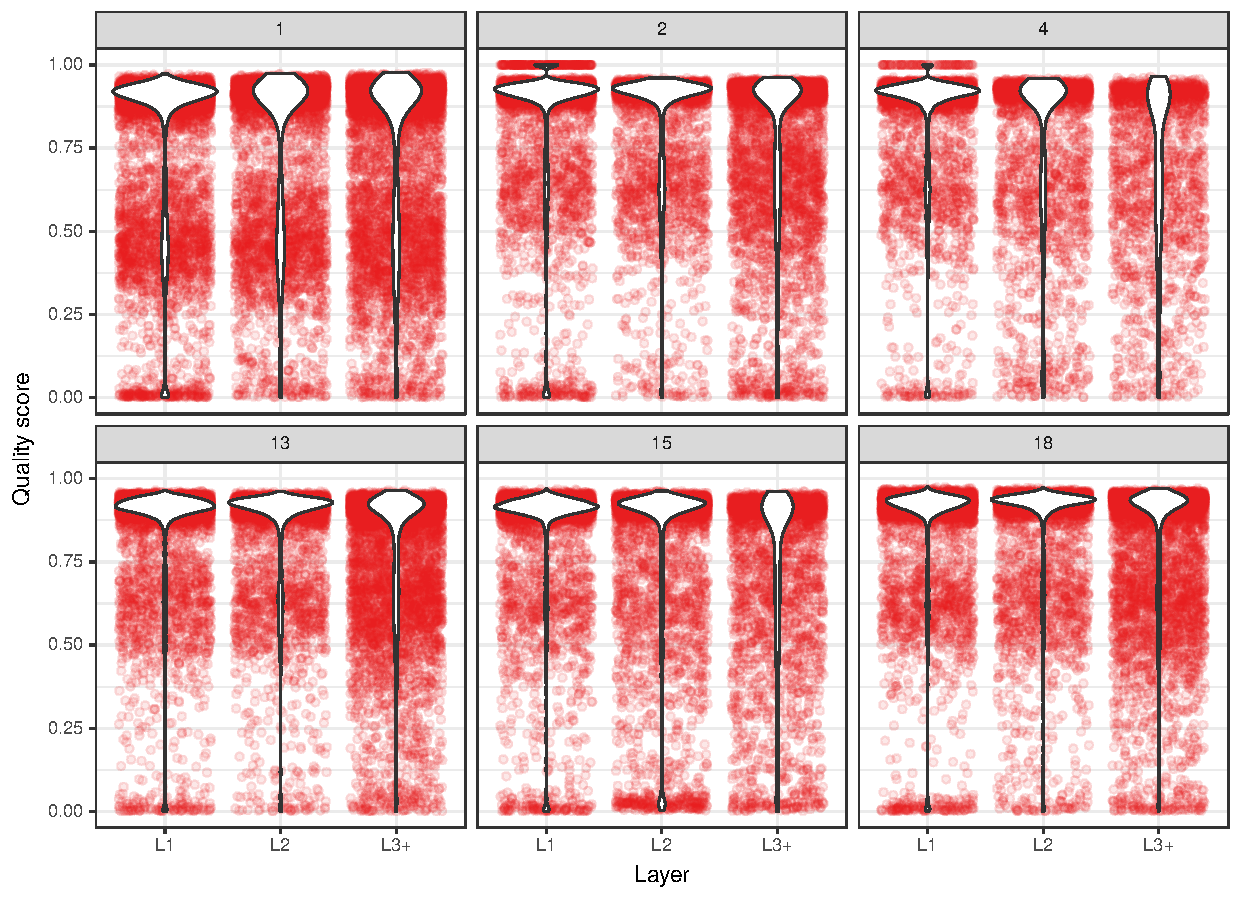
\includegraphics[width=.95\textwidth]{tracking_quality_layer.pdf}
        \centering
        \includegraphics[width=.95\textwidth]{tracking_quality_time.pdf} % second figure itself
        \caption[Tracking quality]{Quality distributions per plant, layer, and timepoint
          for all plants.
        Some timepoints have distributions scoring in the $\sim$1 regime, which
        corresponds to situations where the automatic tracking failed. These
        timepoints have been manually tracked for cells in the L1 within 30
        $\mu$m of the topmost CLV3 expressing cell.}
      \label{fig:tracking_quality}
\end{figure}
The data tracking quality is defined as the F1 score, also known as the
Dice-S{\o}rensen score, between timepoints. The
F1 score gives an appreciation of the overall accuracy of a test on the form of
\begin{equation}
  F_1 = 2 \frac{precision\times recall}{precision + recall},
  \label{eq:f1}
\end{equation}
i.e.\ as the harmonic mean between precision and recall. It can also be
expressed on set form as 
\begin{equation}
  F_1 = 2 \frac{X_t \cap X_{t+1}}{X_t \cup X_{t+1}}
  \label{eq:f1_set}
\end{equation}
where $X_t$ denotes the set in question in timepoint $t$. In other words, the more cells are
contained between timepoints, the higher the F1 score.

As \cref{fig:tracking_quality} shows, the quality for the tracking is overall
relatively high, with only a few timepoints having bigger clusters with low F1
scores. These cells are however typically positioned at the periphery of the
SAM, at the very edges of the segmentation, and are therefore both of lesser
interest and importance for the dynamics of the stem cell niche. As described in
\cref{sec:filtering}, we have in all of our analyses excluded the tracking of
cells whose F1 scores are less than $0.30$. The errors in tracking occasionally
causes one cell to be recognized as more than two in the next timeframe. In
these cases, we choose the two daughter cells by order of tracking quality.

That timepoints 40 and 48 hours in plant 2, as well as timepoint 20 hours in
plant 4 have perfect F1 scores is due to the tracking procedure failing at
these points. The tracking has therefore been manually corrected for the cells
within $30\mu$m of the highest CLV3 expressing cell.

\section{Segmentation quality}
\label{sec:data_errors_segmentation}
While holding an overall excellent quality, the data contains several types
of segmentation errors. For both the  
nuclear and the membrane segmentation, this typically takes the form of basins
of attraction identified as either one when there in fact are multiple, or
multiple when there is in fact only one. In particular, this causes errors with
respect to the apprciation of membrane and nuclear volumes. It also indirectly
affects the tracking quality, as clumped cells in one timepoint can lead to an
erroneously identified division event in the next, in case the segmentation
becomes correct. 

Segmentation errors are however the most prevalent in the peripheral regions of
the SAM, and with deeper penetration into the tissue. Generally, the membrane
segmentation holds higher quality than the nuclear one, where the latter
degrades quickly after deeper penetration than the L2. The overall quality is
also decreasing with the distance from the apex, although to a minor extent in
the L1. 

\begin{figure}[H]
  \centering
  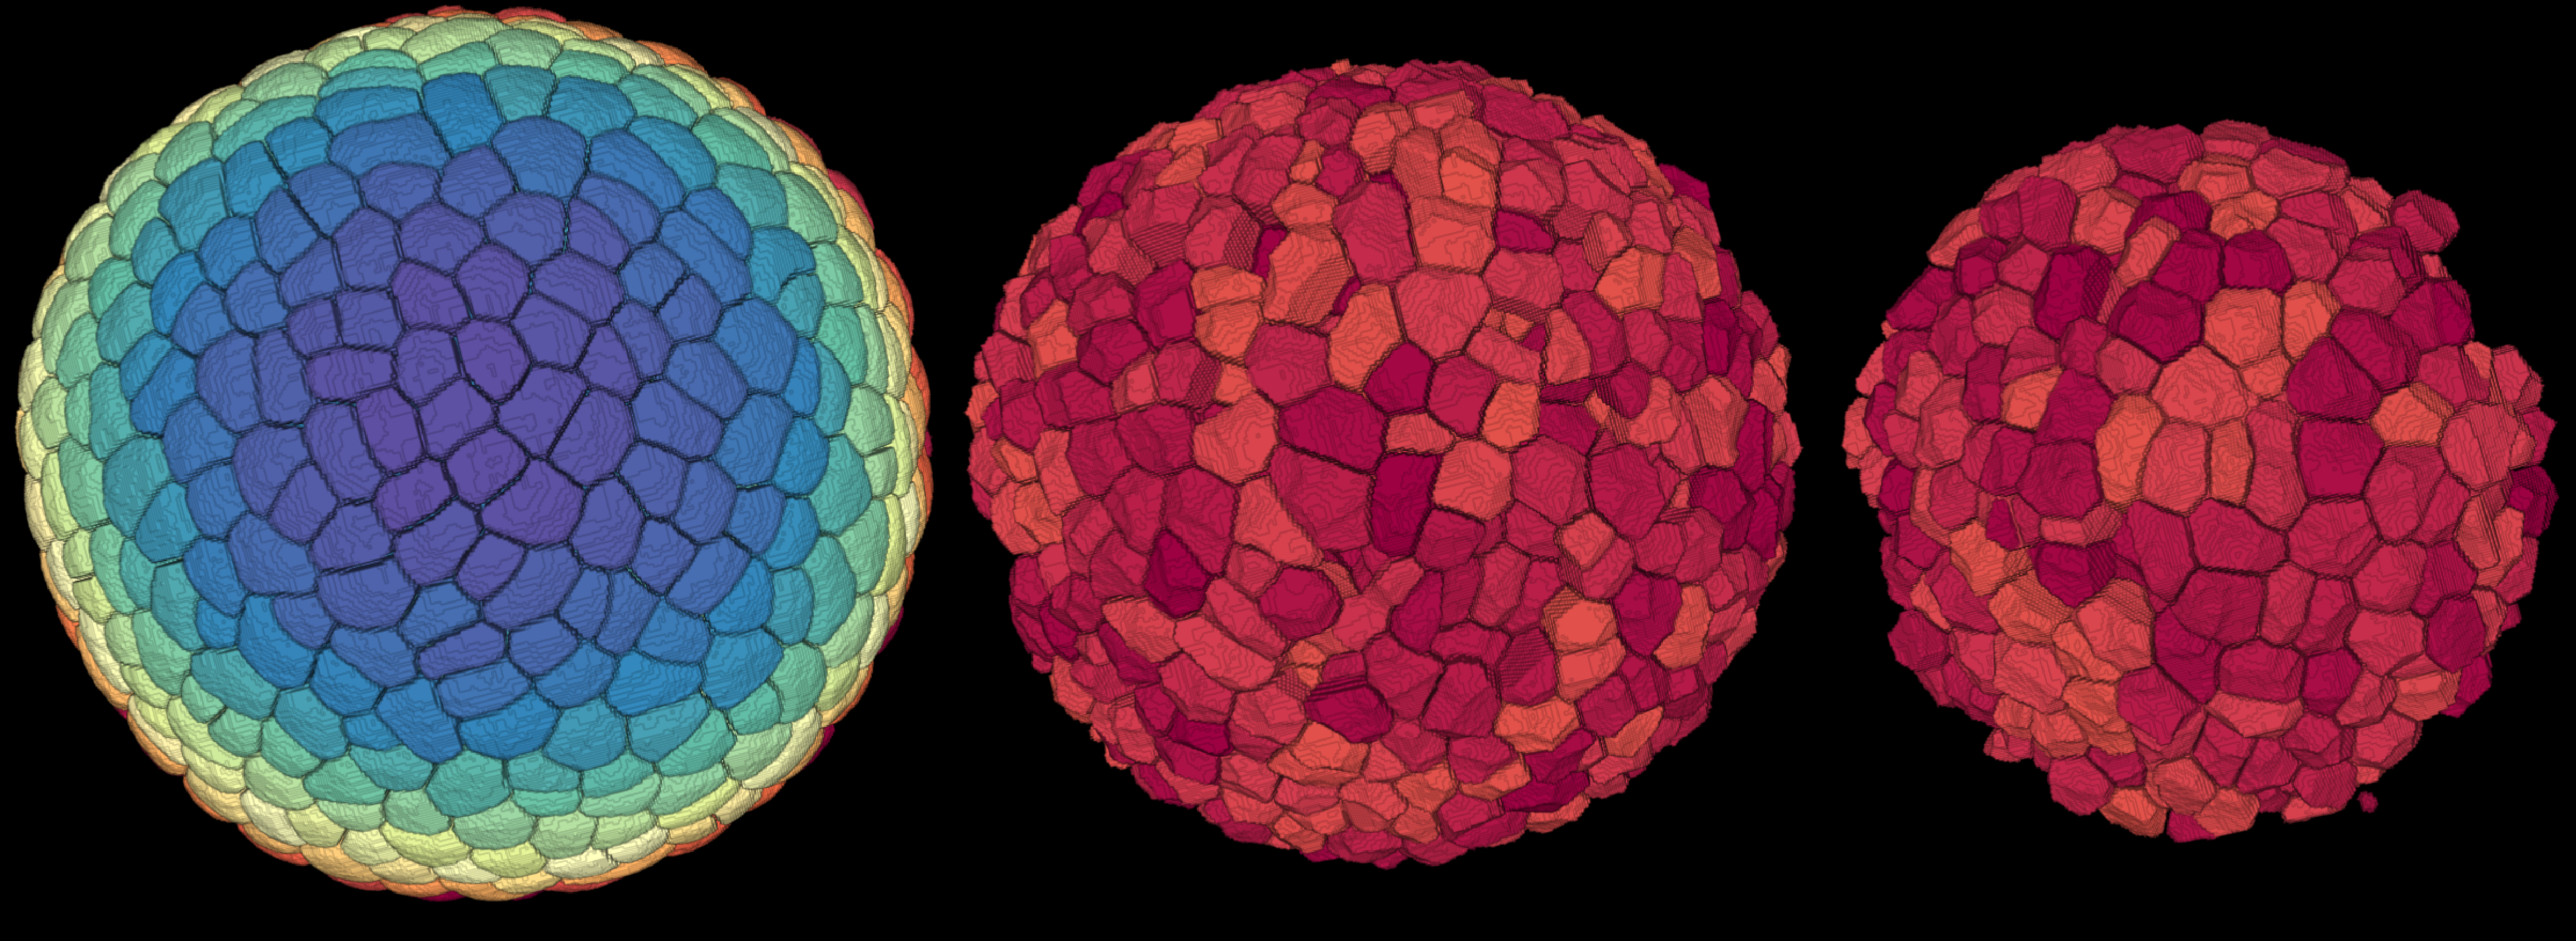
\includegraphics[width=\textwidth]{layer_quality_segm.pdf}
  \caption[Membrane segmentation quality per layer]{Membrane segmentation
    quality separated into L1, L2 and L3 respectively. L1 shows a smooth upper
    surface with well-segmented cells. Also L2 and L3 show high segmentation
    quality, but with a rougher surface to the cells being restricted by the
    cell layer on top, causing a ruggedness in the cell surface. Note in
    particular how the quality in the periphery of the SAM generally are of
    lesser quality, with occasional cell remnants being identified as actual
    cells, e.g.\ in the bottom right.}
  \label{fig:layer_quality_segm}
\end{figure}

Generally, the overall quality for the membrane segmentation is high in all
three layers, as shown in \cref{fig:layer_quality_segm}, although the number of errors increase with deeper tissue
penetration. For the nuclear segmentation, mostly cells from the L1 and L2 are
sufficiently reliable, with declining quality with larger distance to the CZ.
The errors with multiply matching nuclei are occurring mostly in the subepidermal
cells, and in those cases largely in the peripheral regions.

\section{Missing timepoints}
\label{sec:missingtp}
The dataset contains several missing timepoints in the nuclear and membrane
data. As previously noted, plant 1 and 18 lacks all timepoints for the nuclear
data, whereas plant 4 and 15 lack nuclear data for timepoints 24 and 12 hours
respectively. Plant 18 also lacks data for timepoint 40 hours.


%!TEX root = ../thesis.tex
% ******************************* Thesis Appendix B ********************************

\chapter{This is an appendix}


\end{appendices}

% *************************************** Index ********************************
\printthesisindex % If index is present

\end{document}
